\documentclass[a4paper]{article}
\usepackage[utf8]{inputenc}
\usepackage{tikz}
\usetikzlibrary{positioning}
\usepackage{graphicx}
\usepackage{hyperref}
\usepackage{amsmath}
\numberwithin{equation}{section}
%\usepackage{rotating}
%\usepackage{subfig}
%\usepackage{nth}
%\usepackage{amsmath}
%\usepackage{float}
\usepackage[parfill]{parskip}
%\usepackage[top=1in, bottom=1in, left=1in, right=1in]{geometry}
%\usepackage[T1S]{fontenc}
\usepackage[nottoc,numbib]{tocbibind} % To make the references show in the ToC

\DeclareUnicodeCharacter{00A0}{ }

\title{Indirect Online Evolution of Neural Features} % TODO better title?

\author{Martin \textsc{Gammelsæter} -- \texttt{martin.gammelsaeter@epfl.ch}}
\date{2014-12-26}

\begin{document}
\maketitle

\tableofcontents
\newpage

\topskip0pt
\vspace*{\fill}
\section{Summary}
TODO
\vspace*{\fill}
\newpage

\topskip0pt
\vspace*{\fill}
\section{Project description}

% TODO clean up "we" vs "them" etc

A recent publication by Auerbach, Fernando and Floreano \cite{auerbach2014online}
introduced the idea of using competing "neuronal replicators" to aid in solving
a supervised learning task. Here, the units of replication are individual
hidden units of an artificial neural network (ANN) that is actively learning
from a stream of data, similar to a robot acting in the world. In that
publication, the utility of this neuronal replication was showed on a toy
problem with some simplifications (binary inputs, binary hidden unit
activations, uniformly distributed inputs), but we would like to extend this
method to more complex, real-world problems where those simplifications are
relaxed. This project will involve extending the existing system to perform on
more complex problems. This will involve first implementing an indirect
encoding for the feature weights so that larger dimensional problems are
evolvable. The next step will involve a lot of experimentation with
parameters, fitness functions, diversity mechanisms, etc to discover a setup
that can (hopefully) outperform other online learning frameworks.

\vspace*{\fill}
\newpage

\section{Introduction}
In some situations, using machine learning methods which learn incrementally
from experience -- online machine learning methods -- is preferable. One such
situation is robotics, in which it is often benefitial to gradually learn the
target function through interaction with the environment, as well as being able
to respond to \emph{changes} in this possibly dynamic environment. This is as
opposed to using offline learning, in which the learning algorithm is presented
with a finite set of examples from which to train and generalize. Such offline
methods are rarely able to adapt to dynamic enviroments, and generally useless
if a sizeable set of training examples is not available ahead of time.
Auerbach, Fernando and Floreano \cite{auerbach2014online} recently proposed a
new online learning method, called \emph{Online Evolutionary Extreme Learning
Machines} (OEELMs), based on the concepts of \emph{Extreme Learning Machines}
(ELMs) \cite{huang2012extreme}, the neural replicator hypothesis
\cite{fernando2010neuronal}, and earlier work by Mahmood and Sutton
\cite{mahmood2013representation}. The method will be more rigorously described
later in this report. Roughly however, OEELMs works by letting the hidden
features in a neural net be individuals in an evolutionary algorithm, where the
fitness is measured as each feature's contribution to the output. Badly
performing features are then ``killed'' and replaced by new features which are
the product of the classical evolutionary algorithm operators such as mutation
and crossover. Such an algorithm is called a steady-state evolutionary
algorithm \cite{back2000evolutionary}.

OEELMs were shown to work better than other methods when learning a simple
random function with 20 inputs in \cite{auerbach2014online}. But, as the result
section of this report will show, the use of evolution does not improve the
performance of the algorithm over simply using a static set of random features
when trying to learn a much more complex problem like the MNIST dataset of
handwritten digits \cite{lecun1998gradient}. In short, this project attempts to
extend the OEELM method to use an indirect encoding scheme called
\emph{HyperNEAT} \cite{stanley2009hypercube} to improve the effectiveness of
OEELMs.

TODO WHAT IS THE CONCLUSION, IN ONE SENTENCE?

\section{Theoretical background}

\subsection{Online Evolutionary Extreme Learning Machines}
As mentioned in both the project description and the introduction, OEELMs were
introduced by Auerbach, Fernando, and Floreano at the \emph{Artificial Life}
conference in 2014 \cite{auerbach2014online}. The origin comes from the ELMs of
Huang et al.\ \cite{huang2012extreme}. This work formalizes a
single-hidden-layer feed-forward neural network in which the input weights to
the hidden features are stochastically assigned and unchanged throughout
training, leaving only the output weights to be trained -- a linear regression
problem. An illustration of the network can be seen in Fig.~\ref{fig:elm}.
Huang et al. show that the ELMs are able to outperform popular supervised
regression and classification techniques such as some \emph{Support Vector
Machine} (SVM) variants. This work was extended by Mahmood and Sutton
\cite{mahmood2013representation}, showing that in an online version of the ELM
algorithm, accuracy can be enhanced by a selectionist approach where one
regularly drops badly performing features as measured by their contributions to
the output (i.e.\ the magnitude of the weight(s) between that feature and the
output neurons). The dropped features are then replaced by new stochastically
generated features, hoping that they will perform better than the features they
replace.

\begin{figure}
    \centering
    % Graphic for TeX using PGF
% Title: /home/mg/Diagram1.dia
% Creator: Dia v0.97.2
% CreationDate: Sat Dec 27 16:05:49 2014
% For: mg
% \usepackage{tikz}
% The following commands are not supported in PSTricks at present
% We define them conditionally, so when they are implemented,
% this pgf file will use them.
\ifx\du\undefined
  \newlength{\du}
\fi
\setlength{\du}{15\unitlength}
\begin{tikzpicture}
\pgftransformxscale{1.000000}
\pgftransformyscale{-1.000000}
\definecolor{dialinecolor}{rgb}{0.000000, 0.000000, 0.000000}
\pgfsetstrokecolor{dialinecolor}
\definecolor{dialinecolor}{rgb}{1.000000, 1.000000, 1.000000}
\pgfsetfillcolor{dialinecolor}
\pgfsetlinewidth{0.100000\du}
\pgfsetdash{}{0pt}
\pgfsetdash{}{0pt}
\pgfsetbuttcap
\pgfsetmiterjoin
\pgfsetlinewidth{0.100000\du}
\pgfsetbuttcap
\pgfsetmiterjoin
\pgfsetdash{}{0pt}
\definecolor{dialinecolor}{rgb}{1.000000, 1.000000, 1.000000}
\pgfsetfillcolor{dialinecolor}
\pgfpathellipse{\pgfpoint{6.350000\du}{6.350000\du}}{\pgfpoint{1.350000\du}{0\du}}{\pgfpoint{0\du}{1.350000\du}}
\pgfusepath{fill}
\definecolor{dialinecolor}{rgb}{0.000000, 0.000000, 0.000000}
\pgfsetstrokecolor{dialinecolor}
\pgfpathellipse{\pgfpoint{6.350000\du}{6.350000\du}}{\pgfpoint{1.350000\du}{0\du}}{\pgfpoint{0\du}{1.350000\du}}
\pgfusepath{stroke}
\pgfsetbuttcap
\pgfsetmiterjoin
\pgfsetdash{}{0pt}
\definecolor{dialinecolor}{rgb}{0.000000, 0.000000, 0.000000}
\pgfsetstrokecolor{dialinecolor}
\pgfpathellipse{\pgfpoint{6.350000\du}{6.350000\du}}{\pgfpoint{1.350000\du}{0\du}}{\pgfpoint{0\du}{1.350000\du}}
\pgfusepath{stroke}
\pgfsetlinewidth{0.100000\du}
\pgfsetdash{}{0pt}
\pgfsetdash{}{0pt}
\pgfsetbuttcap
\pgfsetmiterjoin
\pgfsetlinewidth{0.100000\du}
\pgfsetbuttcap
\pgfsetmiterjoin
\pgfsetdash{}{0pt}
\definecolor{dialinecolor}{rgb}{1.000000, 1.000000, 1.000000}
\pgfsetfillcolor{dialinecolor}
\pgfpathellipse{\pgfpoint{6.350000\du}{13.350000\du}}{\pgfpoint{1.350000\du}{0\du}}{\pgfpoint{0\du}{1.350000\du}}
\pgfusepath{fill}
\definecolor{dialinecolor}{rgb}{0.000000, 0.000000, 0.000000}
\pgfsetstrokecolor{dialinecolor}
\pgfpathellipse{\pgfpoint{6.350000\du}{13.350000\du}}{\pgfpoint{1.350000\du}{0\du}}{\pgfpoint{0\du}{1.350000\du}}
\pgfusepath{stroke}
\pgfsetbuttcap
\pgfsetmiterjoin
\pgfsetdash{}{0pt}
\definecolor{dialinecolor}{rgb}{0.000000, 0.000000, 0.000000}
\pgfsetstrokecolor{dialinecolor}
\pgfpathellipse{\pgfpoint{6.350000\du}{13.350000\du}}{\pgfpoint{1.350000\du}{0\du}}{\pgfpoint{0\du}{1.350000\du}}
\pgfusepath{stroke}
\pgfsetlinewidth{0.100000\du}
\pgfsetdash{}{0pt}
\pgfsetdash{}{0pt}
\pgfsetbuttcap
\pgfsetmiterjoin
\pgfsetlinewidth{0.100000\du}
\pgfsetbuttcap
\pgfsetmiterjoin
\pgfsetdash{}{0pt}
\definecolor{dialinecolor}{rgb}{0.000000, 0.000000, 0.000000}
\pgfsetfillcolor{dialinecolor}
\pgfpathellipse{\pgfpoint{6.350000\du}{8.650000\du}}{\pgfpoint{0.150000\du}{0\du}}{\pgfpoint{0\du}{0.150000\du}}
\pgfusepath{fill}
\definecolor{dialinecolor}{rgb}{0.000000, 0.000000, 0.000000}
\pgfsetstrokecolor{dialinecolor}
\pgfpathellipse{\pgfpoint{6.350000\du}{8.650000\du}}{\pgfpoint{0.150000\du}{0\du}}{\pgfpoint{0\du}{0.150000\du}}
\pgfusepath{stroke}
\pgfsetbuttcap
\pgfsetmiterjoin
\pgfsetdash{}{0pt}
\definecolor{dialinecolor}{rgb}{0.000000, 0.000000, 0.000000}
\pgfsetstrokecolor{dialinecolor}
\pgfpathellipse{\pgfpoint{6.350000\du}{8.650000\du}}{\pgfpoint{0.150000\du}{0\du}}{\pgfpoint{0\du}{0.150000\du}}
\pgfusepath{stroke}
\pgfsetlinewidth{0.100000\du}
\pgfsetdash{}{0pt}
\pgfsetdash{}{0pt}
\pgfsetbuttcap
\pgfsetmiterjoin
\pgfsetlinewidth{0.100000\du}
\pgfsetbuttcap
\pgfsetmiterjoin
\pgfsetdash{}{0pt}
\definecolor{dialinecolor}{rgb}{0.000000, 0.000000, 0.000000}
\pgfsetfillcolor{dialinecolor}
\pgfpathellipse{\pgfpoint{6.350000\du}{9.750000\du}}{\pgfpoint{0.150000\du}{0\du}}{\pgfpoint{0\du}{0.150000\du}}
\pgfusepath{fill}
\definecolor{dialinecolor}{rgb}{0.000000, 0.000000, 0.000000}
\pgfsetstrokecolor{dialinecolor}
\pgfpathellipse{\pgfpoint{6.350000\du}{9.750000\du}}{\pgfpoint{0.150000\du}{0\du}}{\pgfpoint{0\du}{0.150000\du}}
\pgfusepath{stroke}
\pgfsetbuttcap
\pgfsetmiterjoin
\pgfsetdash{}{0pt}
\definecolor{dialinecolor}{rgb}{0.000000, 0.000000, 0.000000}
\pgfsetstrokecolor{dialinecolor}
\pgfpathellipse{\pgfpoint{6.350000\du}{9.750000\du}}{\pgfpoint{0.150000\du}{0\du}}{\pgfpoint{0\du}{0.150000\du}}
\pgfusepath{stroke}
\pgfsetlinewidth{0.100000\du}
\pgfsetdash{}{0pt}
\pgfsetdash{}{0pt}
\pgfsetbuttcap
\pgfsetmiterjoin
\pgfsetlinewidth{0.100000\du}
\pgfsetbuttcap
\pgfsetmiterjoin
\pgfsetdash{}{0pt}
\definecolor{dialinecolor}{rgb}{0.000000, 0.000000, 0.000000}
\pgfsetfillcolor{dialinecolor}
\pgfpathellipse{\pgfpoint{6.350000\du}{10.850000\du}}{\pgfpoint{0.150000\du}{0\du}}{\pgfpoint{0\du}{0.150000\du}}
\pgfusepath{fill}
\definecolor{dialinecolor}{rgb}{0.000000, 0.000000, 0.000000}
\pgfsetstrokecolor{dialinecolor}
\pgfpathellipse{\pgfpoint{6.350000\du}{10.850000\du}}{\pgfpoint{0.150000\du}{0\du}}{\pgfpoint{0\du}{0.150000\du}}
\pgfusepath{stroke}
\pgfsetbuttcap
\pgfsetmiterjoin
\pgfsetdash{}{0pt}
\definecolor{dialinecolor}{rgb}{0.000000, 0.000000, 0.000000}
\pgfsetstrokecolor{dialinecolor}
\pgfpathellipse{\pgfpoint{6.350000\du}{10.850000\du}}{\pgfpoint{0.150000\du}{0\du}}{\pgfpoint{0\du}{0.150000\du}}
\pgfusepath{stroke}
\pgfsetlinewidth{0.100000\du}
\pgfsetdash{}{0pt}
\pgfsetdash{}{0pt}
\pgfsetbuttcap
\pgfsetmiterjoin
\pgfsetlinewidth{0.100000\du}
\pgfsetbuttcap
\pgfsetmiterjoin
\pgfsetdash{}{0pt}
\definecolor{dialinecolor}{rgb}{1.000000, 1.000000, 1.000000}
\pgfsetfillcolor{dialinecolor}
\pgfpathellipse{\pgfpoint{19.242987\du}{9.598368\du}}{\pgfpoint{1.350000\du}{0\du}}{\pgfpoint{0\du}{1.350000\du}}
\pgfusepath{fill}
\definecolor{dialinecolor}{rgb}{0.000000, 0.000000, 0.000000}
\pgfsetstrokecolor{dialinecolor}
\pgfpathellipse{\pgfpoint{19.242987\du}{9.598368\du}}{\pgfpoint{1.350000\du}{0\du}}{\pgfpoint{0\du}{1.350000\du}}
\pgfusepath{stroke}
\pgfsetbuttcap
\pgfsetmiterjoin
\pgfsetdash{}{0pt}
\definecolor{dialinecolor}{rgb}{0.000000, 0.000000, 0.000000}
\pgfsetstrokecolor{dialinecolor}
\pgfpathellipse{\pgfpoint{19.242987\du}{9.598368\du}}{\pgfpoint{1.350000\du}{0\du}}{\pgfpoint{0\du}{1.350000\du}}
\pgfusepath{stroke}
\pgfsetlinewidth{0.100000\du}
\pgfsetdash{}{0pt}
\pgfsetdash{}{0pt}
\pgfsetbuttcap
\pgfsetmiterjoin
\pgfsetlinewidth{0.100000\du}
\pgfsetbuttcap
\pgfsetmiterjoin
\pgfsetdash{}{0pt}
\definecolor{dialinecolor}{rgb}{1.000000, 1.000000, 1.000000}
\pgfsetfillcolor{dialinecolor}
\pgfpathellipse{\pgfpoint{12.350000\du}{8.350000\du}}{\pgfpoint{1.350000\du}{0\du}}{\pgfpoint{0\du}{1.350000\du}}
\pgfusepath{fill}
\definecolor{dialinecolor}{rgb}{0.000000, 0.000000, 0.000000}
\pgfsetstrokecolor{dialinecolor}
\pgfpathellipse{\pgfpoint{12.350000\du}{8.350000\du}}{\pgfpoint{1.350000\du}{0\du}}{\pgfpoint{0\du}{1.350000\du}}
\pgfusepath{stroke}
\pgfsetbuttcap
\pgfsetmiterjoin
\pgfsetdash{}{0pt}
\definecolor{dialinecolor}{rgb}{0.000000, 0.000000, 0.000000}
\pgfsetstrokecolor{dialinecolor}
\pgfpathellipse{\pgfpoint{12.350000\du}{8.350000\du}}{\pgfpoint{1.350000\du}{0\du}}{\pgfpoint{0\du}{1.350000\du}}
\pgfusepath{stroke}
\pgfsetlinewidth{0.100000\du}
\pgfsetdash{}{0pt}
\pgfsetdash{}{0pt}
\pgfsetbuttcap
\pgfsetmiterjoin
\pgfsetlinewidth{0.100000\du}
\pgfsetbuttcap
\pgfsetmiterjoin
\pgfsetdash{}{0pt}
\definecolor{dialinecolor}{rgb}{1.000000, 1.000000, 1.000000}
\pgfsetfillcolor{dialinecolor}
\pgfpathellipse{\pgfpoint{12.350000\du}{15.350000\du}}{\pgfpoint{1.350000\du}{0\du}}{\pgfpoint{0\du}{1.350000\du}}
\pgfusepath{fill}
\definecolor{dialinecolor}{rgb}{0.000000, 0.000000, 0.000000}
\pgfsetstrokecolor{dialinecolor}
\pgfpathellipse{\pgfpoint{12.350000\du}{15.350000\du}}{\pgfpoint{1.350000\du}{0\du}}{\pgfpoint{0\du}{1.350000\du}}
\pgfusepath{stroke}
\pgfsetbuttcap
\pgfsetmiterjoin
\pgfsetdash{}{0pt}
\definecolor{dialinecolor}{rgb}{0.000000, 0.000000, 0.000000}
\pgfsetstrokecolor{dialinecolor}
\pgfpathellipse{\pgfpoint{12.350000\du}{15.350000\du}}{\pgfpoint{1.350000\du}{0\du}}{\pgfpoint{0\du}{1.350000\du}}
\pgfusepath{stroke}
\pgfsetlinewidth{0.100000\du}
\pgfsetdash{}{0pt}
\pgfsetdash{}{0pt}
\pgfsetbuttcap
\pgfsetmiterjoin
\pgfsetlinewidth{0.100000\du}
\pgfsetbuttcap
\pgfsetmiterjoin
\pgfsetdash{}{0pt}
\definecolor{dialinecolor}{rgb}{0.000000, 0.000000, 0.000000}
\pgfsetfillcolor{dialinecolor}
\pgfpathellipse{\pgfpoint{12.350000\du}{10.650000\du}}{\pgfpoint{0.150000\du}{0\du}}{\pgfpoint{0\du}{0.150000\du}}
\pgfusepath{fill}
\definecolor{dialinecolor}{rgb}{0.000000, 0.000000, 0.000000}
\pgfsetstrokecolor{dialinecolor}
\pgfpathellipse{\pgfpoint{12.350000\du}{10.650000\du}}{\pgfpoint{0.150000\du}{0\du}}{\pgfpoint{0\du}{0.150000\du}}
\pgfusepath{stroke}
\pgfsetbuttcap
\pgfsetmiterjoin
\pgfsetdash{}{0pt}
\definecolor{dialinecolor}{rgb}{0.000000, 0.000000, 0.000000}
\pgfsetstrokecolor{dialinecolor}
\pgfpathellipse{\pgfpoint{12.350000\du}{10.650000\du}}{\pgfpoint{0.150000\du}{0\du}}{\pgfpoint{0\du}{0.150000\du}}
\pgfusepath{stroke}
\pgfsetlinewidth{0.100000\du}
\pgfsetdash{}{0pt}
\pgfsetdash{}{0pt}
\pgfsetbuttcap
\pgfsetmiterjoin
\pgfsetlinewidth{0.100000\du}
\pgfsetbuttcap
\pgfsetmiterjoin
\pgfsetdash{}{0pt}
\definecolor{dialinecolor}{rgb}{0.000000, 0.000000, 0.000000}
\pgfsetfillcolor{dialinecolor}
\pgfpathellipse{\pgfpoint{12.350000\du}{11.750000\du}}{\pgfpoint{0.150000\du}{0\du}}{\pgfpoint{0\du}{0.150000\du}}
\pgfusepath{fill}
\definecolor{dialinecolor}{rgb}{0.000000, 0.000000, 0.000000}
\pgfsetstrokecolor{dialinecolor}
\pgfpathellipse{\pgfpoint{12.350000\du}{11.750000\du}}{\pgfpoint{0.150000\du}{0\du}}{\pgfpoint{0\du}{0.150000\du}}
\pgfusepath{stroke}
\pgfsetbuttcap
\pgfsetmiterjoin
\pgfsetdash{}{0pt}
\definecolor{dialinecolor}{rgb}{0.000000, 0.000000, 0.000000}
\pgfsetstrokecolor{dialinecolor}
\pgfpathellipse{\pgfpoint{12.350000\du}{11.750000\du}}{\pgfpoint{0.150000\du}{0\du}}{\pgfpoint{0\du}{0.150000\du}}
\pgfusepath{stroke}
\pgfsetlinewidth{0.100000\du}
\pgfsetdash{}{0pt}
\pgfsetdash{}{0pt}
\pgfsetbuttcap
\pgfsetmiterjoin
\pgfsetlinewidth{0.100000\du}
\pgfsetbuttcap
\pgfsetmiterjoin
\pgfsetdash{}{0pt}
\definecolor{dialinecolor}{rgb}{0.000000, 0.000000, 0.000000}
\pgfsetfillcolor{dialinecolor}
\pgfpathellipse{\pgfpoint{12.350000\du}{12.850000\du}}{\pgfpoint{0.150000\du}{0\du}}{\pgfpoint{0\du}{0.150000\du}}
\pgfusepath{fill}
\definecolor{dialinecolor}{rgb}{0.000000, 0.000000, 0.000000}
\pgfsetstrokecolor{dialinecolor}
\pgfpathellipse{\pgfpoint{12.350000\du}{12.850000\du}}{\pgfpoint{0.150000\du}{0\du}}{\pgfpoint{0\du}{0.150000\du}}
\pgfusepath{stroke}
\pgfsetbuttcap
\pgfsetmiterjoin
\pgfsetdash{}{0pt}
\definecolor{dialinecolor}{rgb}{0.000000, 0.000000, 0.000000}
\pgfsetstrokecolor{dialinecolor}
\pgfpathellipse{\pgfpoint{12.350000\du}{12.850000\du}}{\pgfpoint{0.150000\du}{0\du}}{\pgfpoint{0\du}{0.150000\du}}
\pgfusepath{stroke}
\pgfsetlinewidth{0.100000\du}
\pgfsetdash{}{0pt}
\pgfsetdash{}{0pt}
\pgfsetbuttcap
\pgfsetmiterjoin
\pgfsetlinewidth{0.100000\du}
\pgfsetbuttcap
\pgfsetmiterjoin
\pgfsetdash{}{0pt}
\definecolor{dialinecolor}{rgb}{1.000000, 1.000000, 1.000000}
\pgfsetfillcolor{dialinecolor}
\pgfpathellipse{\pgfpoint{12.350000\du}{4.350000\du}}{\pgfpoint{1.350000\du}{0\du}}{\pgfpoint{0\du}{1.350000\du}}
\pgfusepath{fill}
\definecolor{dialinecolor}{rgb}{0.000000, 0.000000, 0.000000}
\pgfsetstrokecolor{dialinecolor}
\pgfpathellipse{\pgfpoint{12.350000\du}{4.350000\du}}{\pgfpoint{1.350000\du}{0\du}}{\pgfpoint{0\du}{1.350000\du}}
\pgfusepath{stroke}
\pgfsetbuttcap
\pgfsetmiterjoin
\pgfsetdash{}{0pt}
\definecolor{dialinecolor}{rgb}{0.000000, 0.000000, 0.000000}
\pgfsetstrokecolor{dialinecolor}
\pgfpathellipse{\pgfpoint{12.350000\du}{4.350000\du}}{\pgfpoint{1.350000\du}{0\du}}{\pgfpoint{0\du}{1.350000\du}}
\pgfusepath{stroke}
\pgfsetlinewidth{0.100000\du}
\pgfsetdash{}{0pt}
\pgfsetdash{}{0pt}
\pgfsetbuttcap
{
\definecolor{dialinecolor}{rgb}{0.000000, 0.000000, 0.000000}
\pgfsetfillcolor{dialinecolor}
% was here!!!
\pgfsetarrowsend{to}
\definecolor{dialinecolor}{rgb}{0.000000, 0.000000, 0.000000}
\pgfsetstrokecolor{dialinecolor}
\draw (7.700000\du,6.350000\du)--(11.000000\du,4.350000\du);
}
\pgfsetlinewidth{0.100000\du}
\pgfsetdash{}{0pt}
\pgfsetdash{}{0pt}
\pgfsetbuttcap
{
\definecolor{dialinecolor}{rgb}{0.000000, 0.000000, 0.000000}
\pgfsetfillcolor{dialinecolor}
% was here!!!
\pgfsetarrowsend{to}
\definecolor{dialinecolor}{rgb}{0.000000, 0.000000, 0.000000}
\pgfsetstrokecolor{dialinecolor}
\draw (7.700000\du,13.350000\du)--(11.000000\du,4.350000\du);
}
\pgfsetlinewidth{0.100000\du}
\pgfsetdash{}{0pt}
\pgfsetdash{}{0pt}
\pgfsetbuttcap
{
\definecolor{dialinecolor}{rgb}{0.000000, 0.000000, 0.000000}
\pgfsetfillcolor{dialinecolor}
% was here!!!
\pgfsetarrowsend{to}
\definecolor{dialinecolor}{rgb}{0.000000, 0.000000, 0.000000}
\pgfsetstrokecolor{dialinecolor}
\draw (7.700000\du,6.350000\du)--(11.000000\du,8.350000\du);
}
\pgfsetlinewidth{0.100000\du}
\pgfsetdash{}{0pt}
\pgfsetdash{}{0pt}
\pgfsetbuttcap
{
\definecolor{dialinecolor}{rgb}{0.000000, 0.000000, 0.000000}
\pgfsetfillcolor{dialinecolor}
% was here!!!
\pgfsetarrowsend{to}
\definecolor{dialinecolor}{rgb}{0.000000, 0.000000, 0.000000}
\pgfsetstrokecolor{dialinecolor}
\draw (7.700000\du,6.350000\du)--(11.000000\du,15.350000\du);
}
\pgfsetlinewidth{0.100000\du}
\pgfsetdash{}{0pt}
\pgfsetdash{}{0pt}
\pgfsetbuttcap
{
\definecolor{dialinecolor}{rgb}{0.000000, 0.000000, 0.000000}
\pgfsetfillcolor{dialinecolor}
% was here!!!
\pgfsetarrowsend{to}
\definecolor{dialinecolor}{rgb}{0.000000, 0.000000, 0.000000}
\pgfsetstrokecolor{dialinecolor}
\draw (7.700000\du,13.350000\du)--(11.000000\du,8.350000\du);
}
\pgfsetlinewidth{0.100000\du}
\pgfsetdash{}{0pt}
\pgfsetdash{}{0pt}
\pgfsetbuttcap
{
\definecolor{dialinecolor}{rgb}{0.000000, 0.000000, 0.000000}
\pgfsetfillcolor{dialinecolor}
% was here!!!
\pgfsetarrowsend{to}
\definecolor{dialinecolor}{rgb}{0.000000, 0.000000, 0.000000}
\pgfsetstrokecolor{dialinecolor}
\draw (7.700000\du,13.350000\du)--(11.000000\du,15.350000\du);
}
\pgfsetlinewidth{0.100000\du}
\pgfsetdash{}{0pt}
\pgfsetdash{}{0pt}
\pgfsetbuttcap
{
\definecolor{dialinecolor}{rgb}{0.000000, 0.000000, 0.000000}
\pgfsetfillcolor{dialinecolor}
% was here!!!
\pgfsetarrowsend{to}
\definecolor{dialinecolor}{rgb}{0.000000, 0.000000, 0.000000}
\pgfsetstrokecolor{dialinecolor}
\draw (13.700000\du,4.350000\du)--(17.892987\du,9.598368\du);
}
\pgfsetlinewidth{0.100000\du}
\pgfsetdash{}{0pt}
\pgfsetdash{}{0pt}
\pgfsetbuttcap
{
\definecolor{dialinecolor}{rgb}{0.000000, 0.000000, 0.000000}
\pgfsetfillcolor{dialinecolor}
% was here!!!
\pgfsetarrowsend{to}
\definecolor{dialinecolor}{rgb}{0.000000, 0.000000, 0.000000}
\pgfsetstrokecolor{dialinecolor}
\draw (13.700000\du,8.350000\du)--(17.892987\du,9.598368\du);
}
\pgfsetlinewidth{0.100000\du}
\pgfsetdash{}{0pt}
\pgfsetdash{}{0pt}
\pgfsetbuttcap
{
\definecolor{dialinecolor}{rgb}{0.000000, 0.000000, 0.000000}
\pgfsetfillcolor{dialinecolor}
% was here!!!
\pgfsetarrowsend{to}
\definecolor{dialinecolor}{rgb}{0.000000, 0.000000, 0.000000}
\pgfsetstrokecolor{dialinecolor}
\draw (13.700000\du,15.350000\du)--(17.892987\du,9.598368\du);
}
% setfont left to latex
\definecolor{dialinecolor}{rgb}{0.000000, 0.000000, 0.000000}
\pgfsetstrokecolor{dialinecolor}
\node[anchor=west] at (7.000000\du,2.000000\du){};
% setfont left to latex
\definecolor{dialinecolor}{rgb}{0.000000, 0.000000, 0.000000}
\pgfsetstrokecolor{dialinecolor}
\node[anchor=west] at (4.906847\du,3.126133\du){Inputs};
% setfont left to latex
\definecolor{dialinecolor}{rgb}{0.000000, 0.000000, 0.000000}
\pgfsetstrokecolor{dialinecolor}
\node[anchor=west] at (11.000000\du,1.957956\du){Features};
% setfont left to latex
\definecolor{dialinecolor}{rgb}{0.000000, 0.000000, 0.000000}
\pgfsetstrokecolor{dialinecolor}
\node[anchor=west] at (17.915911\du,6.531724\du){Outputs};
\pgfsetlinewidth{0.200000\du}
\pgfsetdash{}{0pt}
\pgfsetdash{}{0pt}
\pgfsetbuttcap
{
\definecolor{dialinecolor}{rgb}{0.000000, 0.000000, 0.000000}
\pgfsetfillcolor{dialinecolor}
% was here!!!
\pgfsetarrowsend{to}
\definecolor{dialinecolor}{rgb}{0.000000, 0.000000, 0.000000}
\pgfsetstrokecolor{dialinecolor}
\draw (7.000000\du,18.000000\du)--(9.000000\du,15.000000\du);
}
% setfont left to latex
\definecolor{dialinecolor}{rgb}{0.000000, 0.000000, 0.000000}
\pgfsetstrokecolor{dialinecolor}
\node[anchor=west] at (5.135197\du,18.873867\du){Feature weights};
\pgfsetlinewidth{0.200000\du}
\pgfsetdash{}{0pt}
\pgfsetdash{}{0pt}
\pgfsetbuttcap
{
\definecolor{dialinecolor}{rgb}{0.000000, 0.000000, 0.000000}
\pgfsetfillcolor{dialinecolor}
% was here!!!
\pgfsetarrowsend{to}
\definecolor{dialinecolor}{rgb}{0.000000, 0.000000, 0.000000}
\pgfsetstrokecolor{dialinecolor}
\draw (17.000000\du,16.000000\du)--(16.579557\du,12.831823\du);
}
% setfont left to latex
\definecolor{dialinecolor}{rgb}{0.000000, 0.000000, 0.000000}
\pgfsetstrokecolor{dialinecolor}
\node[anchor=west] at (15.570493\du,16.915911\du){Output weights};
\end{tikzpicture}

    \caption{The basic ELM feed-forward network. Feature weights are
    stochastically generated, and only the output weights are updated through
    training}
    \label{fig:elm}
\end{figure}

Auerbach et al.\ further extends Mahmood and Sutton's work by instead of simply
replacing the dropped features by new stochastically generated features, they
use the concepts of evolutionary algorithms to replace dropped features with
features that are guided by artificial evolution. This idea is inspired by the
neural replicator hypothesis \cite{fernando2010neuronal}, which hypothesizes
that ``replication (with mutation) of patterns of neuronal activity can occur
within the brain using known neurophysiological processes''. If this is true, it
means that the concept of evolution influences brains not only in the
development, but also within the lifetime of an individual. Auerbach et al.\
uses a very simple evolutionary algorithm where the genotypes are simply binary
strings that directly encodes the (binary) input weights to the feature that
that genotype represents. In every iteration, for every feature to be replaced
(a settable parameter), a binary tournament between two randomly chosen
remaining features are conducted where the feature with the highest fitness
(magnitude of output weight) wins. The fitness is calculated in the following
way
\begin{equation}
    fitness(f) = \lvert w_{f \rightarrow o} \rvert
    \label{eq:oeelmfitness}
\end{equation}
where $f$ is the feature evaluated, and $w_{f \rightarrow o}$ is the connection
weight between $f$ and the output $o$. After the fitness evaluation, the
winning feature is copied, and every gene is mutated with some probability
$p_{mutate}$. This mutated copy then replaces the dropped feature.

The weights of the features are updated every iteration in an online fashion:
\begin{equation}
    \forall f \,(\Delta w_{f \rightarrow o} = \eta \times err \times v_f)
    \label{eq:oeelmdeltaw}
\end{equation}
where $\eta$ is the learning rate, $err$ is the difference between the network's
output and the correct output, and $v_f$ is the output from the feature $f$.

Because of the very simple evolutionary mechanism, perhaps inspired by the
simplicity of the hypothesized mechanisms for evolution in the neural replicator
hypothesis, there is no computational overhead over the selectionist method.
Because of the binary tournament, the computational cost of the procedure is no
more than the cost of creating a new random feature: $O(m)$ where $m$ is the
number of dimensions in the input. In the paper they show that this evolutionary
approach yields better results than the selectionist approach when approximating
a simple random function (a stochastically initialized feed forward neural
network) with 20 binary inputs. However, as the complexity of the random
function is increased (by increasing the number of hidden features in the random
network), the improvement seen diminishes and disappears.

\subsection{NeuroEvolution of Augmented Topologies}
\emph{NeuroEvolution of Augmented Topologies}, or NEAT, is a genetic algorithm
for generating artificial neural networks proposed by Stanley and Miikkulainen
in 2002 \cite{stanley2002evolving}. It is an indirect encoding -- as opposed to
a direct encoding, where the weights (and possibly topology) of the network are
all simply encoded as single genes that represent a specific weight. It works
by starting with a population of small, simple networks, typically without a
hidden layer. Throughout evolution, the networks are mutated in different ways,
like mutating the weights (like in direct encodings) and adding new neurons.
Increasing genome length like this is a phenomenon also encountered in real
natural evolution \cite{martin1999increasing}. Another important concept is the
concept of speciation within the algorithm. NEAT allows many different
``species'' to coexist within the population. The intuition behind this is that
adding new structure is usually not instantly advantageous, but since
individuals mostly compete against other individuals within its species, new
large structural changes are protected for a while, and are able to optimize
their behaviour before they have to compete with the remaining population.

\begin{figure}[ht]
    \centering
    % Graphic for TeX using PGF
% Title: /home/mg/dev/NEAT-OEELM/report/figs/CPPNnet.dia
% Creator: Dia v0.97.2
% CreationDate: Sun Dec 28 12:41:15 2014
% For: mg
% \usepackage{tikz}
% The following commands are not supported in PSTricks at present
% We define them conditionally, so when they are implemented,
% this pgf file will use them.
\ifx\du\undefined
  \newlength{\du}
\fi
\setlength{\du}{15\unitlength}
\begin{tikzpicture}
\pgftransformxscale{1.000000}
\pgftransformyscale{-1.000000}
\definecolor{dialinecolor}{rgb}{0.000000, 0.000000, 0.000000}
\pgfsetstrokecolor{dialinecolor}
\definecolor{dialinecolor}{rgb}{1.000000, 1.000000, 1.000000}
\pgfsetfillcolor{dialinecolor}
\pgfsetlinewidth{0.100000\du}
\pgfsetdash{}{0pt}
\pgfsetdash{}{0pt}
\pgfsetbuttcap
\pgfsetmiterjoin
\pgfsetlinewidth{0.100000\du}
\pgfsetbuttcap
\pgfsetmiterjoin
\pgfsetdash{}{0pt}
\definecolor{dialinecolor}{rgb}{1.000000, 1.000000, 1.000000}
\pgfsetfillcolor{dialinecolor}
\fill (8.000000\du,14.000000\du)--(8.000000\du,16.000000\du)--(10.000000\du,16.000000\du)--(10.000000\du,14.000000\du)--cycle;
\definecolor{dialinecolor}{rgb}{0.000000, 0.000000, 0.000000}
\pgfsetstrokecolor{dialinecolor}
\draw (8.000000\du,14.000000\du)--(8.000000\du,16.000000\du)--(10.000000\du,16.000000\du)--(10.000000\du,14.000000\du)--cycle;
\pgfsetlinewidth{0.050000\du}
\pgfsetbuttcap
\pgfsetmiterjoin
\pgfsetdash{}{0pt}
\definecolor{dialinecolor}{rgb}{0.752941, 0.752941, 0.752941}
\pgfsetstrokecolor{dialinecolor}
\draw (9.000000\du,14.200000\du)--(9.000000\du,15.800000\du);
\pgfsetbuttcap
\pgfsetmiterjoin
\pgfsetdash{}{0pt}
\definecolor{dialinecolor}{rgb}{0.752941, 0.752941, 0.752941}
\pgfsetstrokecolor{dialinecolor}
\draw (8.200000\du,15.000000\du)--(9.800000\du,15.000000\du);
\pgfsetlinewidth{0.100000\du}
\pgfsetbuttcap
\pgfsetmiterjoin
\pgfsetdash{}{0pt}
\definecolor{dialinecolor}{rgb}{0.000000, 0.000000, 0.000000}
\pgfsetstrokecolor{dialinecolor}
\pgfpathmoveto{\pgfpoint{8.200000\du}{15.000000\du}}
\pgfpathcurveto{\pgfpoint{8.200000\du}{15.000000\du}}{\pgfpoint{8.400000\du}{15.600000\du}}{\pgfpoint{8.600000\du}{15.600000\du}}
\pgfpathcurveto{\pgfpoint{8.800000\du}{15.600000\du}}{\pgfpoint{9.200000\du}{14.400000\du}}{\pgfpoint{9.400000\du}{14.400000\du}}
\pgfpathcurveto{\pgfpoint{9.600000\du}{14.400000\du}}{\pgfpoint{9.800000\du}{15.000000\du}}{\pgfpoint{9.800000\du}{15.000000\du}}
\pgfusepath{stroke}
\pgfsetlinewidth{0.100000\du}
\pgfsetdash{}{0pt}
\pgfsetdash{}{0pt}
\pgfsetbuttcap
\pgfsetmiterjoin
\pgfsetlinewidth{0.100000\du}
\pgfsetbuttcap
\pgfsetmiterjoin
\pgfsetdash{}{0pt}
\definecolor{dialinecolor}{rgb}{1.000000, 1.000000, 1.000000}
\pgfsetfillcolor{dialinecolor}
\fill (8.000000\du,10.000000\du)--(8.000000\du,12.000000\du)--(10.000000\du,12.000000\du)--(10.000000\du,10.000000\du)--cycle;
\definecolor{dialinecolor}{rgb}{0.000000, 0.000000, 0.000000}
\pgfsetstrokecolor{dialinecolor}
\draw (8.000000\du,10.000000\du)--(8.000000\du,12.000000\du)--(10.000000\du,12.000000\du)--(10.000000\du,10.000000\du)--cycle;
\pgfsetlinewidth{0.050000\du}
\pgfsetbuttcap
\pgfsetmiterjoin
\pgfsetdash{}{0pt}
\definecolor{dialinecolor}{rgb}{0.752941, 0.752941, 0.752941}
\pgfsetstrokecolor{dialinecolor}
\draw (9.000000\du,10.200000\du)--(9.000000\du,11.800000\du);
\pgfsetbuttcap
\pgfsetmiterjoin
\pgfsetdash{}{0pt}
\definecolor{dialinecolor}{rgb}{0.752941, 0.752941, 0.752941}
\pgfsetstrokecolor{dialinecolor}
\draw (8.200000\du,11.000000\du)--(9.800000\du,11.000000\du);
\pgfsetlinewidth{0.100000\du}
\pgfsetbuttcap
\pgfsetmiterjoin
\pgfsetdash{}{0pt}
\definecolor{dialinecolor}{rgb}{0.000000, 0.000000, 0.000000}
\pgfsetstrokecolor{dialinecolor}
\pgfpathmoveto{\pgfpoint{8.200000\du}{11.800000\du}}
\pgfpathcurveto{\pgfpoint{9.400000\du}{11.800000\du}}{\pgfpoint{8.600000\du}{10.200000\du}}{\pgfpoint{9.800000\du}{10.200000\du}}
\pgfusepath{stroke}
\pgfsetlinewidth{0.100000\du}
\pgfsetdash{}{0pt}
\pgfsetdash{}{0pt}
\pgfsetbuttcap
\pgfsetmiterjoin
\pgfsetlinewidth{0.100000\du}
\pgfsetbuttcap
\pgfsetmiterjoin
\pgfsetdash{}{0pt}
\definecolor{dialinecolor}{rgb}{1.000000, 1.000000, 1.000000}
\pgfsetfillcolor{dialinecolor}
\fill (12.000000\du,14.000000\du)--(12.000000\du,16.000000\du)--(14.000000\du,16.000000\du)--(14.000000\du,14.000000\du)--cycle;
\definecolor{dialinecolor}{rgb}{0.000000, 0.000000, 0.000000}
\pgfsetstrokecolor{dialinecolor}
\draw (12.000000\du,14.000000\du)--(12.000000\du,16.000000\du)--(14.000000\du,16.000000\du)--(14.000000\du,14.000000\du)--cycle;
\pgfsetlinewidth{0.050000\du}
\pgfsetbuttcap
\pgfsetmiterjoin
\pgfsetdash{}{0pt}
\definecolor{dialinecolor}{rgb}{0.752941, 0.752941, 0.752941}
\pgfsetstrokecolor{dialinecolor}
\draw (13.000000\du,14.200000\du)--(13.000000\du,15.800000\du);
\pgfsetbuttcap
\pgfsetmiterjoin
\pgfsetdash{}{0pt}
\definecolor{dialinecolor}{rgb}{0.752941, 0.752941, 0.752941}
\pgfsetstrokecolor{dialinecolor}
\draw (12.200000\du,15.000000\du)--(13.800000\du,15.000000\du);
\pgfsetlinewidth{0.100000\du}
\pgfsetbuttcap
\pgfsetmiterjoin
\pgfsetdash{}{0pt}
\definecolor{dialinecolor}{rgb}{0.000000, 0.000000, 0.000000}
\pgfsetstrokecolor{dialinecolor}
\draw (12.400000\du,15.000000\du)--(13.000000\du,15.000000\du)--(13.000000\du,14.400000\du)--(13.600000\du,14.400000\du);
\pgfsetlinewidth{0.100000\du}
\pgfsetdash{}{0pt}
\pgfsetdash{}{0pt}
\pgfsetbuttcap
\pgfsetmiterjoin
\pgfsetlinewidth{0.100000\du}
\pgfsetbuttcap
\pgfsetmiterjoin
\pgfsetdash{}{0pt}
\definecolor{dialinecolor}{rgb}{1.000000, 1.000000, 1.000000}
\pgfsetfillcolor{dialinecolor}
\fill (10.000000\du,6.000000\du)--(10.000000\du,8.000000\du)--(12.000000\du,8.000000\du)--(12.000000\du,6.000000\du)--cycle;
\definecolor{dialinecolor}{rgb}{0.000000, 0.000000, 0.000000}
\pgfsetstrokecolor{dialinecolor}
\draw (10.000000\du,6.000000\du)--(10.000000\du,8.000000\du)--(12.000000\du,8.000000\du)--(12.000000\du,6.000000\du)--cycle;
\pgfsetlinewidth{0.050000\du}
\pgfsetbuttcap
\pgfsetmiterjoin
\pgfsetdash{}{0pt}
\definecolor{dialinecolor}{rgb}{0.752941, 0.752941, 0.752941}
\pgfsetstrokecolor{dialinecolor}
\draw (11.000000\du,6.200000\du)--(11.000000\du,7.800000\du);
\pgfsetbuttcap
\pgfsetmiterjoin
\pgfsetdash{}{0pt}
\definecolor{dialinecolor}{rgb}{0.752941, 0.752941, 0.752941}
\pgfsetstrokecolor{dialinecolor}
\draw (10.200000\du,7.000000\du)--(11.800000\du,7.000000\du);
\pgfsetlinewidth{0.100000\du}
\pgfsetbuttcap
\pgfsetmiterjoin
\pgfsetdash{}{0pt}
\definecolor{dialinecolor}{rgb}{0.000000, 0.000000, 0.000000}
\pgfsetstrokecolor{dialinecolor}
\draw (10.200000\du,7.200000\du)--(11.800000\du,6.800000\du);
\pgfsetlinewidth{0.100000\du}
\pgfsetdash{}{0pt}
\pgfsetdash{}{0pt}
\pgfsetbuttcap
{
\definecolor{dialinecolor}{rgb}{0.000000, 0.000000, 0.000000}
\pgfsetfillcolor{dialinecolor}
% was here!!!
\pgfsetarrowsend{to}
\definecolor{dialinecolor}{rgb}{0.000000, 0.000000, 0.000000}
\pgfsetstrokecolor{dialinecolor}
\draw (9.000000\du,14.000000\du)--(9.000000\du,12.000000\du);
}
\pgfsetlinewidth{0.100000\du}
\pgfsetdash{}{0pt}
\pgfsetdash{}{0pt}
\pgfsetbuttcap
{
\definecolor{dialinecolor}{rgb}{0.000000, 0.000000, 0.000000}
\pgfsetfillcolor{dialinecolor}
% was here!!!
\pgfsetarrowsend{to}
\definecolor{dialinecolor}{rgb}{0.000000, 0.000000, 0.000000}
\pgfsetstrokecolor{dialinecolor}
\draw (13.000000\du,14.000000\du)--(11.000000\du,8.000000\du);
}
\pgfsetlinewidth{0.100000\du}
\pgfsetdash{}{0pt}
\pgfsetdash{}{0pt}
\pgfsetbuttcap
{
\definecolor{dialinecolor}{rgb}{0.000000, 0.000000, 0.000000}
\pgfsetfillcolor{dialinecolor}
% was here!!!
\pgfsetarrowsend{to}
\definecolor{dialinecolor}{rgb}{0.000000, 0.000000, 0.000000}
\pgfsetstrokecolor{dialinecolor}
\draw (9.000000\du,10.000000\du)--(11.000000\du,8.000000\du);
}
\pgfsetlinewidth{0.100000\du}
\pgfsetdash{}{0pt}
\pgfsetdash{}{0pt}
\pgfsetbuttcap
{
\definecolor{dialinecolor}{rgb}{0.000000, 0.000000, 0.000000}
\pgfsetfillcolor{dialinecolor}
% was here!!!
\pgfsetarrowsend{to}
\definecolor{dialinecolor}{rgb}{0.000000, 0.000000, 0.000000}
\pgfsetstrokecolor{dialinecolor}
\draw (11.000000\du,6.000000\du)--(11.000000\du,4.000000\du);
}
\pgfsetlinewidth{0.100000\du}
\pgfsetdash{}{0pt}
\pgfsetdash{}{0pt}
\pgfsetbuttcap
{
\definecolor{dialinecolor}{rgb}{0.000000, 0.000000, 0.000000}
\pgfsetfillcolor{dialinecolor}
% was here!!!
\pgfsetarrowsend{to}
\definecolor{dialinecolor}{rgb}{0.000000, 0.000000, 0.000000}
\pgfsetstrokecolor{dialinecolor}
\draw (9.000000\du,18.000000\du)--(9.000000\du,16.000000\du);
}
\pgfsetlinewidth{0.100000\du}
\pgfsetdash{}{0pt}
\pgfsetdash{}{0pt}
\pgfsetbuttcap
{
\definecolor{dialinecolor}{rgb}{0.000000, 0.000000, 0.000000}
\pgfsetfillcolor{dialinecolor}
% was here!!!
\pgfsetarrowsend{to}
\definecolor{dialinecolor}{rgb}{0.000000, 0.000000, 0.000000}
\pgfsetstrokecolor{dialinecolor}
\draw (13.000000\du,18.000000\du)--(13.000000\du,16.000000\du);
}
\pgfsetlinewidth{0.100000\du}
\pgfsetdash{}{0pt}
\pgfsetdash{}{0pt}
\pgfsetbuttcap
{
\definecolor{dialinecolor}{rgb}{0.000000, 0.000000, 0.000000}
\pgfsetfillcolor{dialinecolor}
% was here!!!
\pgfsetarrowsend{to}
\definecolor{dialinecolor}{rgb}{0.000000, 0.000000, 0.000000}
\pgfsetstrokecolor{dialinecolor}
\draw (13.000000\du,18.000000\du)--(9.000000\du,16.000000\du);
}
\pgfsetlinewidth{0.100000\du}
\pgfsetdash{}{0pt}
\pgfsetdash{}{0pt}
\pgfsetbuttcap
{
\definecolor{dialinecolor}{rgb}{0.000000, 0.000000, 0.000000}
\pgfsetfillcolor{dialinecolor}
% was here!!!
\pgfsetarrowsend{to}
\definecolor{dialinecolor}{rgb}{0.000000, 0.000000, 0.000000}
\pgfsetstrokecolor{dialinecolor}
\draw (9.000000\du,18.000000\du)--(13.000000\du,16.000000\du);
}
% setfont left to latex
\definecolor{dialinecolor}{rgb}{0.000000, 0.000000, 0.000000}
\pgfsetstrokecolor{dialinecolor}
\node[anchor=west] at (8.550000\du,19.000000\du){X};
% setfont left to latex
\definecolor{dialinecolor}{rgb}{0.000000, 0.000000, 0.000000}
\pgfsetstrokecolor{dialinecolor}
\node[anchor=west] at (12.600000\du,18.950000\du){Y};
% setfont left to latex
\definecolor{dialinecolor}{rgb}{0.000000, 0.000000, 0.000000}
\pgfsetstrokecolor{dialinecolor}
\node[anchor=west] at (9.700000\du,3.500000\du){Output};
\pgfsetlinewidth{0.100000\du}
\pgfsetdash{}{0pt}
\pgfsetdash{}{0pt}
\pgfsetbuttcap
\pgfsetmiterjoin
\pgfsetlinewidth{0.100000\du}
\pgfsetbuttcap
\pgfsetmiterjoin
\pgfsetdash{}{0pt}
\definecolor{dialinecolor}{rgb}{1.000000, 1.000000, 1.000000}
\pgfsetfillcolor{dialinecolor}
\fill (19.345960\du,13.046516\du)--(19.345960\du,15.986366\du)--(22.190976\du,15.986366\du)--(22.190976\du,13.046516\du)--cycle;
\definecolor{dialinecolor}{rgb}{0.000000, 0.000000, 0.000000}
\pgfsetstrokecolor{dialinecolor}
\draw (19.345960\du,13.046516\du)--(19.345960\du,15.986366\du)--(22.190976\du,15.986366\du)--(22.190976\du,13.046516\du)--cycle;
\pgfsetbuttcap
\pgfsetmiterjoin
\pgfsetdash{}{0pt}
\definecolor{dialinecolor}{rgb}{0.000000, 0.000000, 0.000000}
\pgfsetstrokecolor{dialinecolor}
\draw (19.345960\du,13.046516\du)--(19.345960\du,15.986366\du)--(22.190976\du,15.986366\du)--(22.190976\du,13.046516\du)--cycle;
\pgfsetlinewidth{0.100000\du}
\pgfsetdash{}{0pt}
\pgfsetdash{}{0pt}
\pgfsetbuttcap
{
\definecolor{dialinecolor}{rgb}{0.000000, 0.000000, 0.000000}
\pgfsetfillcolor{dialinecolor}
% was here!!!
\pgfsetarrowsend{to}
\definecolor{dialinecolor}{rgb}{0.000000, 0.000000, 0.000000}
\pgfsetstrokecolor{dialinecolor}
\draw (16.945960\du,13.576776\du)--(19.345960\du,13.563142\du);
}
\pgfsetlinewidth{0.100000\du}
\pgfsetdash{}{0pt}
\pgfsetdash{}{0pt}
\pgfsetbuttcap
{
\definecolor{dialinecolor}{rgb}{0.000000, 0.000000, 0.000000}
\pgfsetfillcolor{dialinecolor}
% was here!!!
\pgfsetarrowsend{to}
\definecolor{dialinecolor}{rgb}{0.000000, 0.000000, 0.000000}
\pgfsetstrokecolor{dialinecolor}
\draw (16.945960\du,15.400000\du)--(19.345960\du,15.386366\du);
}
% setfont left to latex
\definecolor{dialinecolor}{rgb}{0.000000, 0.000000, 0.000000}
\pgfsetstrokecolor{dialinecolor}
\node[anchor=west] at (16.018916\du,13.494594\du){X};
% setfont left to latex
\definecolor{dialinecolor}{rgb}{0.000000, 0.000000, 0.000000}
\pgfsetstrokecolor{dialinecolor}
\node[anchor=west] at (16.048646\du,15.356763\du){Y};
% setfont left to latex
\definecolor{dialinecolor}{rgb}{0.000000, 0.000000, 0.000000}
\pgfsetstrokecolor{dialinecolor}
\node[anchor=west] at (20.322522\du,14.308335\du){f};
\pgfsetlinewidth{0.100000\du}
\pgfsetdash{}{0pt}
\pgfsetdash{}{0pt}
\pgfsetbuttcap
{
\definecolor{dialinecolor}{rgb}{0.000000, 0.000000, 0.000000}
\pgfsetfillcolor{dialinecolor}
% was here!!!
\pgfsetarrowsend{to}
\definecolor{dialinecolor}{rgb}{0.000000, 0.000000, 0.000000}
\pgfsetstrokecolor{dialinecolor}
\draw (22.190976\du,14.516441\du)--(24.220086\du,10.170007\du);
}
\pgfsetlinewidth{0.100000\du}
\pgfsetdash{}{0pt}
\pgfsetdash{}{0pt}
\pgfsetbuttcap
{
\definecolor{dialinecolor}{rgb}{0.000000, 0.000000, 0.000000}
\pgfsetfillcolor{dialinecolor}
% was here!!!
\pgfsetarrowsend{to}
\definecolor{dialinecolor}{rgb}{0.000000, 0.000000, 0.000000}
\pgfsetstrokecolor{dialinecolor}
\draw (22.190976\du,14.516441\du)--(24.190356\du,11.002447\du);
}
\pgfsetlinewidth{0.100000\du}
\pgfsetdash{}{0pt}
\pgfsetdash{}{0pt}
\pgfsetbuttcap
{
\definecolor{dialinecolor}{rgb}{0.000000, 0.000000, 0.000000}
\pgfsetfillcolor{dialinecolor}
% was here!!!
\pgfsetarrowsend{to}
\definecolor{dialinecolor}{rgb}{0.000000, 0.000000, 0.000000}
\pgfsetstrokecolor{dialinecolor}
\draw (22.190976\du,14.516441\du)--(24.200000\du,11.800000\du);
}
\pgfsetlinewidth{0.100000\du}
\pgfsetdash{}{0pt}
\pgfsetdash{}{0pt}
\pgfsetbuttcap
{
\definecolor{dialinecolor}{rgb}{0.000000, 0.000000, 0.000000}
\pgfsetfillcolor{dialinecolor}
% was here!!!
\pgfsetarrowsend{to}
\definecolor{dialinecolor}{rgb}{0.000000, 0.000000, 0.000000}
\pgfsetstrokecolor{dialinecolor}
\draw (22.190976\du,14.516441\du)--(24.700000\du,10.200000\du);
}
\pgfsetlinewidth{0.100000\du}
\pgfsetdash{}{0pt}
\pgfsetdash{}{0pt}
\pgfsetbuttcap
\pgfsetmiterjoin
\pgfsetlinewidth{0.100000\du}
\pgfsetbuttcap
\pgfsetmiterjoin
\pgfsetdash{}{0pt}
\definecolor{dialinecolor}{rgb}{0.000000, 0.000000, 0.000000}
\pgfsetstrokecolor{dialinecolor}
\draw (23.900000\du,10.100000\du)--(23.900000\du,13.991667\du)--(27.666129\du,13.991667\du)--(27.666129\du,10.100000\du)--cycle;
\pgfsetbuttcap
\pgfsetmiterjoin
\pgfsetdash{}{0pt}
\definecolor{dialinecolor}{rgb}{0.000000, 0.000000, 0.000000}
\pgfsetstrokecolor{dialinecolor}
\draw (23.900000\du,10.100000\du)--(23.900000\du,13.991667\du)--(27.666129\du,13.991667\du)--(27.666129\du,10.100000\du)--cycle;
\pgfsetlinewidth{0.100000\du}
\pgfsetdash{{\pgflinewidth}{0.200000\du}}{0cm}
\pgfsetdash{{\pgflinewidth}{0.200000\du}}{0cm}
\pgfsetbuttcap
{
\definecolor{dialinecolor}{rgb}{0.000000, 0.000000, 0.000000}
\pgfsetfillcolor{dialinecolor}
% was here!!!
\pgfsetarrowsend{to}
\definecolor{dialinecolor}{rgb}{0.000000, 0.000000, 0.000000}
\pgfsetstrokecolor{dialinecolor}
\draw (22.190976\du,14.516441\du)--(24.200000\du,12.600000\du);
}
\end{tikzpicture}

    \caption{Left: A simple CPPN, made up of functions like a unsigned step
    function, a sine function, a sigmoid function, and a linear function. Inputs
    are Cartesian coordinates. Right: The CPPN $f$ is queried for each
    coordinate in some plane to generate a mapping}
    \label{fig:cppn}
\end{figure}

In this project, an extension of NEAT that uses \emph{Compositional Pattern
Producing Networks} (CPPNs) is used. CPPNs are networks composed of different
kinds of functions: Periodical functions like sines, symmetrical functions like
gaussians, simple step functions, sigmoids, etcetera. These networks themselves
then represent more complex functions. These functions take Cartesian
coordinates as input, and generate some mapping for each coordinate in a plane
(see Fig.~\ref{fig:cppn} for an illustration).

\subsubsection{rtNEAT}
There are multiple extensions to the NEAT architecture, one of which is used in
this project: Real-time NEAT (rtNEAT), introduced by Stanley et al.\ in 2005
\cite{stanley2005evolving}, was originally used to evolve agents in the
videogame \emph{NERO}. Original NEAT is like most genetic algorithms meant to be
run \emph{offline}, with a generational approach. That is, each individual in
the population is evaluated and given a fitness score, before a new generation
is generated from the old one using evolutionary operators. In rtNEAT however,
one uses a steady-state evolutionary approach, in which one for each ``tick''
drops one feature (usually the one with the lowest fitness), and generates a new
one based on the existing population, which one then has to evaluate the fitness
of before one can tick again. This approach is more like real biological
evolution in that generations coexist, and makes \emph{online} use of the
population feasible.

\subsection{Hypercube-based NEAT}
\emph{Hypercube-based NEAT}, or \emph{HyperNEAT} is a generative, indirect
encoding for evolving neural networks. It was first proposed by Stanley et al.\
in 2009 \cite{stanley2009hypercube}, and uses the NEAT method described above.
Put simply, HyperNEAT uses a population of CPPNs evolved through the NEAT
algorithm to encode the weights of a neural network. Like in
Fig.~\ref{fig:cppn}, the CPPNs are queried with coordinates, where these
coordinates typically represent the position of two different neurons in a
neural \emph{substrate}. Fig.~\ref{fig:substrate} illustrates a typical
HyperNEAT substrate, with an input, hidden, and output layer. Each layer is a
2D-grid, with feed-forward connections between the layers (red lines in the
figure), making the entire substrate 3D. The weights of the connections are set
by the output of a CPPN, where the input is the coordinates of the pre-synaptic
and the post-synaptic neuron. Additionally, one can have other inputs like a
bias, distance to center (to possibly emphasize symmetry around the center)
etcetera.

\begin{figure}[ht]
    \centering
    \resizebox{\textwidth}{!}{% Graphic for TeX using PGF
% Title: /home/mg/dev/NEAT-OEELM/report/figs/substrate.dia
% Creator: Dia v0.97.2
% CreationDate: Sun Dec 28 15:32:41 2014
% For: mg
% \usepackage{tikz}
% The following commands are not supported in PSTricks at present
% We define them conditionally, so when they are implemented,
% this pgf file will use them.
\ifx\du\undefined
  \newlength{\du}
\fi
\setlength{\du}{15\unitlength}
\begin{tikzpicture}
\pgftransformxscale{1.000000}
\pgftransformyscale{-1.000000}
\definecolor{dialinecolor}{rgb}{0.000000, 0.000000, 0.000000}
\pgfsetstrokecolor{dialinecolor}
\definecolor{dialinecolor}{rgb}{1.000000, 1.000000, 1.000000}
\pgfsetfillcolor{dialinecolor}
\pgfsetlinewidth{0.100000\du}
\pgfsetdash{}{0pt}
\pgfsetdash{}{0pt}
\pgfsetbuttcap
\pgfsetmiterjoin
\pgfsetlinewidth{0.100000\du}
\pgfsetbuttcap
\pgfsetmiterjoin
\pgfsetdash{}{0pt}
\definecolor{dialinecolor}{rgb}{1.000000, 1.000000, 1.000000}
\pgfsetfillcolor{dialinecolor}
\pgfpathellipse{\pgfpoint{34.600000\du}{8.600000\du}}{\pgfpoint{1.600000\du}{0\du}}{\pgfpoint{0\du}{1.600000\du}}
\pgfusepath{fill}
\definecolor{dialinecolor}{rgb}{0.000000, 0.000000, 0.000000}
\pgfsetstrokecolor{dialinecolor}
\pgfpathellipse{\pgfpoint{34.600000\du}{8.600000\du}}{\pgfpoint{1.600000\du}{0\du}}{\pgfpoint{0\du}{1.600000\du}}
\pgfusepath{stroke}
\pgfsetbuttcap
\pgfsetmiterjoin
\pgfsetdash{}{0pt}
\definecolor{dialinecolor}{rgb}{0.000000, 0.000000, 0.000000}
\pgfsetstrokecolor{dialinecolor}
\pgfpathellipse{\pgfpoint{34.600000\du}{8.600000\du}}{\pgfpoint{1.600000\du}{0\du}}{\pgfpoint{0\du}{1.600000\du}}
\pgfusepath{stroke}
\pgfsetlinewidth{0.100000\du}
\pgfsetdash{}{0pt}
\pgfsetdash{}{0pt}
\pgfsetbuttcap
\pgfsetmiterjoin
\pgfsetlinewidth{0.100000\du}
\pgfsetbuttcap
\pgfsetmiterjoin
\pgfsetdash{}{0pt}
\definecolor{dialinecolor}{rgb}{1.000000, 1.000000, 1.000000}
\pgfsetfillcolor{dialinecolor}
\pgfpathellipse{\pgfpoint{39.600000\du}{8.600000\du}}{\pgfpoint{1.600000\du}{0\du}}{\pgfpoint{0\du}{1.600000\du}}
\pgfusepath{fill}
\definecolor{dialinecolor}{rgb}{0.000000, 0.000000, 0.000000}
\pgfsetstrokecolor{dialinecolor}
\pgfpathellipse{\pgfpoint{39.600000\du}{8.600000\du}}{\pgfpoint{1.600000\du}{0\du}}{\pgfpoint{0\du}{1.600000\du}}
\pgfusepath{stroke}
\pgfsetbuttcap
\pgfsetmiterjoin
\pgfsetdash{}{0pt}
\definecolor{dialinecolor}{rgb}{0.000000, 0.000000, 0.000000}
\pgfsetstrokecolor{dialinecolor}
\pgfpathellipse{\pgfpoint{39.600000\du}{8.600000\du}}{\pgfpoint{1.600000\du}{0\du}}{\pgfpoint{0\du}{1.600000\du}}
\pgfusepath{stroke}
\pgfsetlinewidth{0.100000\du}
\pgfsetdash{}{0pt}
\pgfsetdash{}{0pt}
\pgfsetbuttcap
\pgfsetmiterjoin
\pgfsetlinewidth{0.100000\du}
\pgfsetbuttcap
\pgfsetmiterjoin
\pgfsetdash{}{0pt}
\definecolor{dialinecolor}{rgb}{1.000000, 1.000000, 1.000000}
\pgfsetfillcolor{dialinecolor}
\pgfpathellipse{\pgfpoint{34.600000\du}{13.600000\du}}{\pgfpoint{1.600000\du}{0\du}}{\pgfpoint{0\du}{1.600000\du}}
\pgfusepath{fill}
\definecolor{dialinecolor}{rgb}{0.000000, 0.000000, 0.000000}
\pgfsetstrokecolor{dialinecolor}
\pgfpathellipse{\pgfpoint{34.600000\du}{13.600000\du}}{\pgfpoint{1.600000\du}{0\du}}{\pgfpoint{0\du}{1.600000\du}}
\pgfusepath{stroke}
\pgfsetbuttcap
\pgfsetmiterjoin
\pgfsetdash{}{0pt}
\definecolor{dialinecolor}{rgb}{0.000000, 0.000000, 0.000000}
\pgfsetstrokecolor{dialinecolor}
\pgfpathellipse{\pgfpoint{34.600000\du}{13.600000\du}}{\pgfpoint{1.600000\du}{0\du}}{\pgfpoint{0\du}{1.600000\du}}
\pgfusepath{stroke}
\pgfsetlinewidth{0.100000\du}
\pgfsetdash{}{0pt}
\pgfsetdash{}{0pt}
\pgfsetbuttcap
\pgfsetmiterjoin
\pgfsetlinewidth{0.100000\du}
\pgfsetbuttcap
\pgfsetmiterjoin
\pgfsetdash{}{0pt}
\definecolor{dialinecolor}{rgb}{1.000000, 1.000000, 1.000000}
\pgfsetfillcolor{dialinecolor}
\pgfpathellipse{\pgfpoint{39.600000\du}{13.600000\du}}{\pgfpoint{1.600000\du}{0\du}}{\pgfpoint{0\du}{1.600000\du}}
\pgfusepath{fill}
\definecolor{dialinecolor}{rgb}{0.000000, 0.000000, 0.000000}
\pgfsetstrokecolor{dialinecolor}
\pgfpathellipse{\pgfpoint{39.600000\du}{13.600000\du}}{\pgfpoint{1.600000\du}{0\du}}{\pgfpoint{0\du}{1.600000\du}}
\pgfusepath{stroke}
\pgfsetbuttcap
\pgfsetmiterjoin
\pgfsetdash{}{0pt}
\definecolor{dialinecolor}{rgb}{0.000000, 0.000000, 0.000000}
\pgfsetstrokecolor{dialinecolor}
\pgfpathellipse{\pgfpoint{39.600000\du}{13.600000\du}}{\pgfpoint{1.600000\du}{0\du}}{\pgfpoint{0\du}{1.600000\du}}
\pgfusepath{stroke}
\pgfsetlinewidth{0.100000\du}
\pgfsetdash{}{0pt}
\pgfsetdash{}{0pt}
\pgfsetbuttcap
\pgfsetmiterjoin
\pgfsetlinewidth{0.100000\du}
\pgfsetbuttcap
\pgfsetmiterjoin
\pgfsetdash{}{0pt}
\definecolor{dialinecolor}{rgb}{1.000000, 1.000000, 1.000000}
\pgfsetfillcolor{dialinecolor}
\pgfpathellipse{\pgfpoint{44.600000\du}{8.600000\du}}{\pgfpoint{1.600000\du}{0\du}}{\pgfpoint{0\du}{1.600000\du}}
\pgfusepath{fill}
\definecolor{dialinecolor}{rgb}{0.000000, 0.000000, 0.000000}
\pgfsetstrokecolor{dialinecolor}
\pgfpathellipse{\pgfpoint{44.600000\du}{8.600000\du}}{\pgfpoint{1.600000\du}{0\du}}{\pgfpoint{0\du}{1.600000\du}}
\pgfusepath{stroke}
\pgfsetbuttcap
\pgfsetmiterjoin
\pgfsetdash{}{0pt}
\definecolor{dialinecolor}{rgb}{0.000000, 0.000000, 0.000000}
\pgfsetstrokecolor{dialinecolor}
\pgfpathellipse{\pgfpoint{44.600000\du}{8.600000\du}}{\pgfpoint{1.600000\du}{0\du}}{\pgfpoint{0\du}{1.600000\du}}
\pgfusepath{stroke}
\pgfsetlinewidth{0.100000\du}
\pgfsetdash{}{0pt}
\pgfsetdash{}{0pt}
\pgfsetbuttcap
\pgfsetmiterjoin
\pgfsetlinewidth{0.100000\du}
\pgfsetbuttcap
\pgfsetmiterjoin
\pgfsetdash{}{0pt}
\definecolor{dialinecolor}{rgb}{1.000000, 1.000000, 1.000000}
\pgfsetfillcolor{dialinecolor}
\pgfpathellipse{\pgfpoint{44.600000\du}{13.600000\du}}{\pgfpoint{1.600000\du}{0\du}}{\pgfpoint{0\du}{1.600000\du}}
\pgfusepath{fill}
\definecolor{dialinecolor}{rgb}{0.000000, 0.000000, 0.000000}
\pgfsetstrokecolor{dialinecolor}
\pgfpathellipse{\pgfpoint{44.600000\du}{13.600000\du}}{\pgfpoint{1.600000\du}{0\du}}{\pgfpoint{0\du}{1.600000\du}}
\pgfusepath{stroke}
\pgfsetbuttcap
\pgfsetmiterjoin
\pgfsetdash{}{0pt}
\definecolor{dialinecolor}{rgb}{0.000000, 0.000000, 0.000000}
\pgfsetstrokecolor{dialinecolor}
\pgfpathellipse{\pgfpoint{44.600000\du}{13.600000\du}}{\pgfpoint{1.600000\du}{0\du}}{\pgfpoint{0\du}{1.600000\du}}
\pgfusepath{stroke}
\pgfsetlinewidth{0.100000\du}
\pgfsetdash{}{0pt}
\pgfsetdash{}{0pt}
\pgfsetbuttcap
\pgfsetmiterjoin
\pgfsetlinewidth{0.100000\du}
\pgfsetbuttcap
\pgfsetmiterjoin
\pgfsetdash{}{0pt}
\definecolor{dialinecolor}{rgb}{1.000000, 1.000000, 1.000000}
\pgfsetfillcolor{dialinecolor}
\pgfpathellipse{\pgfpoint{34.600000\du}{18.600000\du}}{\pgfpoint{1.600000\du}{0\du}}{\pgfpoint{0\du}{1.600000\du}}
\pgfusepath{fill}
\definecolor{dialinecolor}{rgb}{0.000000, 0.000000, 0.000000}
\pgfsetstrokecolor{dialinecolor}
\pgfpathellipse{\pgfpoint{34.600000\du}{18.600000\du}}{\pgfpoint{1.600000\du}{0\du}}{\pgfpoint{0\du}{1.600000\du}}
\pgfusepath{stroke}
\pgfsetbuttcap
\pgfsetmiterjoin
\pgfsetdash{}{0pt}
\definecolor{dialinecolor}{rgb}{0.000000, 0.000000, 0.000000}
\pgfsetstrokecolor{dialinecolor}
\pgfpathellipse{\pgfpoint{34.600000\du}{18.600000\du}}{\pgfpoint{1.600000\du}{0\du}}{\pgfpoint{0\du}{1.600000\du}}
\pgfusepath{stroke}
\pgfsetlinewidth{0.100000\du}
\pgfsetdash{}{0pt}
\pgfsetdash{}{0pt}
\pgfsetbuttcap
\pgfsetmiterjoin
\pgfsetlinewidth{0.100000\du}
\pgfsetbuttcap
\pgfsetmiterjoin
\pgfsetdash{}{0pt}
\definecolor{dialinecolor}{rgb}{1.000000, 1.000000, 1.000000}
\pgfsetfillcolor{dialinecolor}
\pgfpathellipse{\pgfpoint{39.600000\du}{18.600000\du}}{\pgfpoint{1.600000\du}{0\du}}{\pgfpoint{0\du}{1.600000\du}}
\pgfusepath{fill}
\definecolor{dialinecolor}{rgb}{0.000000, 0.000000, 0.000000}
\pgfsetstrokecolor{dialinecolor}
\pgfpathellipse{\pgfpoint{39.600000\du}{18.600000\du}}{\pgfpoint{1.600000\du}{0\du}}{\pgfpoint{0\du}{1.600000\du}}
\pgfusepath{stroke}
\pgfsetbuttcap
\pgfsetmiterjoin
\pgfsetdash{}{0pt}
\definecolor{dialinecolor}{rgb}{0.000000, 0.000000, 0.000000}
\pgfsetstrokecolor{dialinecolor}
\pgfpathellipse{\pgfpoint{39.600000\du}{18.600000\du}}{\pgfpoint{1.600000\du}{0\du}}{\pgfpoint{0\du}{1.600000\du}}
\pgfusepath{stroke}
\pgfsetlinewidth{0.100000\du}
\pgfsetdash{}{0pt}
\pgfsetdash{}{0pt}
\pgfsetbuttcap
\pgfsetmiterjoin
\pgfsetlinewidth{0.100000\du}
\pgfsetbuttcap
\pgfsetmiterjoin
\pgfsetdash{}{0pt}
\definecolor{dialinecolor}{rgb}{1.000000, 1.000000, 1.000000}
\pgfsetfillcolor{dialinecolor}
\pgfpathellipse{\pgfpoint{44.600000\du}{18.600000\du}}{\pgfpoint{1.600000\du}{0\du}}{\pgfpoint{0\du}{1.600000\du}}
\pgfusepath{fill}
\definecolor{dialinecolor}{rgb}{0.000000, 0.000000, 0.000000}
\pgfsetstrokecolor{dialinecolor}
\pgfpathellipse{\pgfpoint{44.600000\du}{18.600000\du}}{\pgfpoint{1.600000\du}{0\du}}{\pgfpoint{0\du}{1.600000\du}}
\pgfusepath{stroke}
\pgfsetbuttcap
\pgfsetmiterjoin
\pgfsetdash{}{0pt}
\definecolor{dialinecolor}{rgb}{0.000000, 0.000000, 0.000000}
\pgfsetstrokecolor{dialinecolor}
\pgfpathellipse{\pgfpoint{44.600000\du}{18.600000\du}}{\pgfpoint{1.600000\du}{0\du}}{\pgfpoint{0\du}{1.600000\du}}
\pgfusepath{stroke}
\pgfsetlinewidth{0.100000\du}
\pgfsetdash{}{0pt}
\pgfsetdash{}{0pt}
\pgfsetbuttcap
\pgfsetmiterjoin
\pgfsetlinewidth{0.100000\du}
\pgfsetbuttcap
\pgfsetmiterjoin
\pgfsetdash{}{0pt}
\definecolor{dialinecolor}{rgb}{1.000000, 1.000000, 1.000000}
\pgfsetfillcolor{dialinecolor}
\pgfpathellipse{\pgfpoint{53.600000\du}{13.600000\du}}{\pgfpoint{1.600000\du}{0\du}}{\pgfpoint{0\du}{1.600000\du}}
\pgfusepath{fill}
\definecolor{dialinecolor}{rgb}{0.000000, 0.000000, 0.000000}
\pgfsetstrokecolor{dialinecolor}
\pgfpathellipse{\pgfpoint{53.600000\du}{13.600000\du}}{\pgfpoint{1.600000\du}{0\du}}{\pgfpoint{0\du}{1.600000\du}}
\pgfusepath{stroke}
\pgfsetbuttcap
\pgfsetmiterjoin
\pgfsetdash{}{0pt}
\definecolor{dialinecolor}{rgb}{0.000000, 0.000000, 0.000000}
\pgfsetstrokecolor{dialinecolor}
\pgfpathellipse{\pgfpoint{53.600000\du}{13.600000\du}}{\pgfpoint{1.600000\du}{0\du}}{\pgfpoint{0\du}{1.600000\du}}
\pgfusepath{stroke}
\pgfsetlinewidth{0.100000\du}
\pgfsetdash{}{0pt}
\pgfsetdash{}{0pt}
\pgfsetbuttcap
\pgfsetmiterjoin
\pgfsetlinewidth{0.100000\du}
\pgfsetbuttcap
\pgfsetmiterjoin
\pgfsetdash{}{0pt}
\definecolor{dialinecolor}{rgb}{1.000000, 1.000000, 1.000000}
\pgfsetfillcolor{dialinecolor}
\pgfpathellipse{\pgfpoint{16.600000\du}{8.600000\du}}{\pgfpoint{1.600000\du}{0\du}}{\pgfpoint{0\du}{1.600000\du}}
\pgfusepath{fill}
\definecolor{dialinecolor}{rgb}{0.000000, 0.000000, 0.000000}
\pgfsetstrokecolor{dialinecolor}
\pgfpathellipse{\pgfpoint{16.600000\du}{8.600000\du}}{\pgfpoint{1.600000\du}{0\du}}{\pgfpoint{0\du}{1.600000\du}}
\pgfusepath{stroke}
\pgfsetbuttcap
\pgfsetmiterjoin
\pgfsetdash{}{0pt}
\definecolor{dialinecolor}{rgb}{0.000000, 0.000000, 0.000000}
\pgfsetstrokecolor{dialinecolor}
\pgfpathellipse{\pgfpoint{16.600000\du}{8.600000\du}}{\pgfpoint{1.600000\du}{0\du}}{\pgfpoint{0\du}{1.600000\du}}
\pgfusepath{stroke}
\pgfsetlinewidth{0.100000\du}
\pgfsetdash{}{0pt}
\pgfsetdash{}{0pt}
\pgfsetbuttcap
\pgfsetmiterjoin
\pgfsetlinewidth{0.100000\du}
\pgfsetbuttcap
\pgfsetmiterjoin
\pgfsetdash{}{0pt}
\definecolor{dialinecolor}{rgb}{1.000000, 1.000000, 1.000000}
\pgfsetfillcolor{dialinecolor}
\pgfpathellipse{\pgfpoint{21.600000\du}{8.600000\du}}{\pgfpoint{1.600000\du}{0\du}}{\pgfpoint{0\du}{1.600000\du}}
\pgfusepath{fill}
\definecolor{dialinecolor}{rgb}{0.000000, 0.000000, 0.000000}
\pgfsetstrokecolor{dialinecolor}
\pgfpathellipse{\pgfpoint{21.600000\du}{8.600000\du}}{\pgfpoint{1.600000\du}{0\du}}{\pgfpoint{0\du}{1.600000\du}}
\pgfusepath{stroke}
\pgfsetbuttcap
\pgfsetmiterjoin
\pgfsetdash{}{0pt}
\definecolor{dialinecolor}{rgb}{0.000000, 0.000000, 0.000000}
\pgfsetstrokecolor{dialinecolor}
\pgfpathellipse{\pgfpoint{21.600000\du}{8.600000\du}}{\pgfpoint{1.600000\du}{0\du}}{\pgfpoint{0\du}{1.600000\du}}
\pgfusepath{stroke}
\pgfsetlinewidth{0.100000\du}
\pgfsetdash{}{0pt}
\pgfsetdash{}{0pt}
\pgfsetbuttcap
\pgfsetmiterjoin
\pgfsetlinewidth{0.100000\du}
\pgfsetbuttcap
\pgfsetmiterjoin
\pgfsetdash{}{0pt}
\definecolor{dialinecolor}{rgb}{1.000000, 1.000000, 1.000000}
\pgfsetfillcolor{dialinecolor}
\pgfpathellipse{\pgfpoint{16.600000\du}{13.600000\du}}{\pgfpoint{1.600000\du}{0\du}}{\pgfpoint{0\du}{1.600000\du}}
\pgfusepath{fill}
\definecolor{dialinecolor}{rgb}{0.000000, 0.000000, 0.000000}
\pgfsetstrokecolor{dialinecolor}
\pgfpathellipse{\pgfpoint{16.600000\du}{13.600000\du}}{\pgfpoint{1.600000\du}{0\du}}{\pgfpoint{0\du}{1.600000\du}}
\pgfusepath{stroke}
\pgfsetbuttcap
\pgfsetmiterjoin
\pgfsetdash{}{0pt}
\definecolor{dialinecolor}{rgb}{0.000000, 0.000000, 0.000000}
\pgfsetstrokecolor{dialinecolor}
\pgfpathellipse{\pgfpoint{16.600000\du}{13.600000\du}}{\pgfpoint{1.600000\du}{0\du}}{\pgfpoint{0\du}{1.600000\du}}
\pgfusepath{stroke}
\pgfsetlinewidth{0.100000\du}
\pgfsetdash{}{0pt}
\pgfsetdash{}{0pt}
\pgfsetbuttcap
\pgfsetmiterjoin
\pgfsetlinewidth{0.100000\du}
\pgfsetbuttcap
\pgfsetmiterjoin
\pgfsetdash{}{0pt}
\definecolor{dialinecolor}{rgb}{1.000000, 1.000000, 1.000000}
\pgfsetfillcolor{dialinecolor}
\pgfpathellipse{\pgfpoint{21.600000\du}{13.600000\du}}{\pgfpoint{1.600000\du}{0\du}}{\pgfpoint{0\du}{1.600000\du}}
\pgfusepath{fill}
\definecolor{dialinecolor}{rgb}{0.000000, 0.000000, 0.000000}
\pgfsetstrokecolor{dialinecolor}
\pgfpathellipse{\pgfpoint{21.600000\du}{13.600000\du}}{\pgfpoint{1.600000\du}{0\du}}{\pgfpoint{0\du}{1.600000\du}}
\pgfusepath{stroke}
\pgfsetbuttcap
\pgfsetmiterjoin
\pgfsetdash{}{0pt}
\definecolor{dialinecolor}{rgb}{0.000000, 0.000000, 0.000000}
\pgfsetstrokecolor{dialinecolor}
\pgfpathellipse{\pgfpoint{21.600000\du}{13.600000\du}}{\pgfpoint{1.600000\du}{0\du}}{\pgfpoint{0\du}{1.600000\du}}
\pgfusepath{stroke}
\pgfsetlinewidth{0.100000\du}
\pgfsetdash{}{0pt}
\pgfsetdash{}{0pt}
\pgfsetbuttcap
\pgfsetmiterjoin
\pgfsetlinewidth{0.100000\du}
\pgfsetbuttcap
\pgfsetmiterjoin
\pgfsetdash{}{0pt}
\definecolor{dialinecolor}{rgb}{1.000000, 1.000000, 1.000000}
\pgfsetfillcolor{dialinecolor}
\pgfpathellipse{\pgfpoint{26.600000\du}{8.600000\du}}{\pgfpoint{1.600000\du}{0\du}}{\pgfpoint{0\du}{1.600000\du}}
\pgfusepath{fill}
\definecolor{dialinecolor}{rgb}{0.000000, 0.000000, 0.000000}
\pgfsetstrokecolor{dialinecolor}
\pgfpathellipse{\pgfpoint{26.600000\du}{8.600000\du}}{\pgfpoint{1.600000\du}{0\du}}{\pgfpoint{0\du}{1.600000\du}}
\pgfusepath{stroke}
\pgfsetbuttcap
\pgfsetmiterjoin
\pgfsetdash{}{0pt}
\definecolor{dialinecolor}{rgb}{0.000000, 0.000000, 0.000000}
\pgfsetstrokecolor{dialinecolor}
\pgfpathellipse{\pgfpoint{26.600000\du}{8.600000\du}}{\pgfpoint{1.600000\du}{0\du}}{\pgfpoint{0\du}{1.600000\du}}
\pgfusepath{stroke}
\pgfsetlinewidth{0.100000\du}
\pgfsetdash{}{0pt}
\pgfsetdash{}{0pt}
\pgfsetbuttcap
\pgfsetmiterjoin
\pgfsetlinewidth{0.100000\du}
\pgfsetbuttcap
\pgfsetmiterjoin
\pgfsetdash{}{0pt}
\definecolor{dialinecolor}{rgb}{1.000000, 1.000000, 1.000000}
\pgfsetfillcolor{dialinecolor}
\pgfpathellipse{\pgfpoint{26.600000\du}{13.600000\du}}{\pgfpoint{1.600000\du}{0\du}}{\pgfpoint{0\du}{1.600000\du}}
\pgfusepath{fill}
\definecolor{dialinecolor}{rgb}{0.000000, 0.000000, 0.000000}
\pgfsetstrokecolor{dialinecolor}
\pgfpathellipse{\pgfpoint{26.600000\du}{13.600000\du}}{\pgfpoint{1.600000\du}{0\du}}{\pgfpoint{0\du}{1.600000\du}}
\pgfusepath{stroke}
\pgfsetbuttcap
\pgfsetmiterjoin
\pgfsetdash{}{0pt}
\definecolor{dialinecolor}{rgb}{0.000000, 0.000000, 0.000000}
\pgfsetstrokecolor{dialinecolor}
\pgfpathellipse{\pgfpoint{26.600000\du}{13.600000\du}}{\pgfpoint{1.600000\du}{0\du}}{\pgfpoint{0\du}{1.600000\du}}
\pgfusepath{stroke}
\pgfsetlinewidth{0.100000\du}
\pgfsetdash{}{0pt}
\pgfsetdash{}{0pt}
\pgfsetbuttcap
\pgfsetmiterjoin
\pgfsetlinewidth{0.100000\du}
\pgfsetbuttcap
\pgfsetmiterjoin
\pgfsetdash{}{0pt}
\definecolor{dialinecolor}{rgb}{1.000000, 1.000000, 1.000000}
\pgfsetfillcolor{dialinecolor}
\pgfpathellipse{\pgfpoint{16.600000\du}{18.600000\du}}{\pgfpoint{1.600000\du}{0\du}}{\pgfpoint{0\du}{1.600000\du}}
\pgfusepath{fill}
\definecolor{dialinecolor}{rgb}{0.000000, 0.000000, 0.000000}
\pgfsetstrokecolor{dialinecolor}
\pgfpathellipse{\pgfpoint{16.600000\du}{18.600000\du}}{\pgfpoint{1.600000\du}{0\du}}{\pgfpoint{0\du}{1.600000\du}}
\pgfusepath{stroke}
\pgfsetbuttcap
\pgfsetmiterjoin
\pgfsetdash{}{0pt}
\definecolor{dialinecolor}{rgb}{0.000000, 0.000000, 0.000000}
\pgfsetstrokecolor{dialinecolor}
\pgfpathellipse{\pgfpoint{16.600000\du}{18.600000\du}}{\pgfpoint{1.600000\du}{0\du}}{\pgfpoint{0\du}{1.600000\du}}
\pgfusepath{stroke}
\pgfsetlinewidth{0.100000\du}
\pgfsetdash{}{0pt}
\pgfsetdash{}{0pt}
\pgfsetbuttcap
\pgfsetmiterjoin
\pgfsetlinewidth{0.100000\du}
\pgfsetbuttcap
\pgfsetmiterjoin
\pgfsetdash{}{0pt}
\definecolor{dialinecolor}{rgb}{1.000000, 1.000000, 1.000000}
\pgfsetfillcolor{dialinecolor}
\pgfpathellipse{\pgfpoint{21.600000\du}{18.600000\du}}{\pgfpoint{1.600000\du}{0\du}}{\pgfpoint{0\du}{1.600000\du}}
\pgfusepath{fill}
\definecolor{dialinecolor}{rgb}{0.000000, 0.000000, 0.000000}
\pgfsetstrokecolor{dialinecolor}
\pgfpathellipse{\pgfpoint{21.600000\du}{18.600000\du}}{\pgfpoint{1.600000\du}{0\du}}{\pgfpoint{0\du}{1.600000\du}}
\pgfusepath{stroke}
\pgfsetbuttcap
\pgfsetmiterjoin
\pgfsetdash{}{0pt}
\definecolor{dialinecolor}{rgb}{0.000000, 0.000000, 0.000000}
\pgfsetstrokecolor{dialinecolor}
\pgfpathellipse{\pgfpoint{21.600000\du}{18.600000\du}}{\pgfpoint{1.600000\du}{0\du}}{\pgfpoint{0\du}{1.600000\du}}
\pgfusepath{stroke}
\pgfsetlinewidth{0.100000\du}
\pgfsetdash{}{0pt}
\pgfsetdash{}{0pt}
\pgfsetbuttcap
\pgfsetmiterjoin
\pgfsetlinewidth{0.100000\du}
\pgfsetbuttcap
\pgfsetmiterjoin
\pgfsetdash{}{0pt}
\definecolor{dialinecolor}{rgb}{1.000000, 1.000000, 1.000000}
\pgfsetfillcolor{dialinecolor}
\pgfpathellipse{\pgfpoint{26.600000\du}{18.600000\du}}{\pgfpoint{1.600000\du}{0\du}}{\pgfpoint{0\du}{1.600000\du}}
\pgfusepath{fill}
\definecolor{dialinecolor}{rgb}{0.000000, 0.000000, 0.000000}
\pgfsetstrokecolor{dialinecolor}
\pgfpathellipse{\pgfpoint{26.600000\du}{18.600000\du}}{\pgfpoint{1.600000\du}{0\du}}{\pgfpoint{0\du}{1.600000\du}}
\pgfusepath{stroke}
\pgfsetbuttcap
\pgfsetmiterjoin
\pgfsetdash{}{0pt}
\definecolor{dialinecolor}{rgb}{0.000000, 0.000000, 0.000000}
\pgfsetstrokecolor{dialinecolor}
\pgfpathellipse{\pgfpoint{26.600000\du}{18.600000\du}}{\pgfpoint{1.600000\du}{0\du}}{\pgfpoint{0\du}{1.600000\du}}
\pgfusepath{stroke}
% setfont left to latex
\definecolor{dialinecolor}{rgb}{0.000000, 0.000000, 0.000000}
\pgfsetstrokecolor{dialinecolor}
\node[anchor=west] at (19.650000\du,5.565426\du){Input layer};
% setfont left to latex
\definecolor{dialinecolor}{rgb}{0.000000, 0.000000, 0.000000}
\pgfsetstrokecolor{dialinecolor}
\node[anchor=west] at (37.400000\du,5.569855\du){Hidden layer};
% setfont left to latex
\definecolor{dialinecolor}{rgb}{0.000000, 0.000000, 0.000000}
\pgfsetstrokecolor{dialinecolor}
\node[anchor=west] at (51.450000\du,10.351587\du){Output layer};
\pgfsetlinewidth{0.100000\du}
\pgfsetdash{}{0pt}
\pgfsetdash{}{0pt}
\pgfsetbuttcap
{
\definecolor{dialinecolor}{rgb}{1.000000, 0.000000, 0.000000}
\pgfsetfillcolor{dialinecolor}
% was here!!!
\definecolor{dialinecolor}{rgb}{1.000000, 0.000000, 0.000000}
\pgfsetstrokecolor{dialinecolor}
\draw (28.200000\du,8.600000\du)--(32.949609\du,8.600000\du);
}
\pgfsetlinewidth{0.100000\du}
\pgfsetdash{}{0pt}
\pgfsetdash{}{0pt}
\pgfsetbuttcap
{
\definecolor{dialinecolor}{rgb}{1.000000, 0.000000, 0.000000}
\pgfsetfillcolor{dialinecolor}
% was here!!!
\definecolor{dialinecolor}{rgb}{1.000000, 0.000000, 0.000000}
\pgfsetstrokecolor{dialinecolor}
\draw (46.200000\du,8.600000\du)--(52.233276\du,12.676538\du);
}
\pgfsetlinewidth{0.100000\du}
\pgfsetdash{}{0pt}
\pgfsetdash{}{0pt}
\pgfsetbuttcap
{
\definecolor{dialinecolor}{rgb}{1.000000, 0.000000, 0.000000}
\pgfsetfillcolor{dialinecolor}
% was here!!!
\definecolor{dialinecolor}{rgb}{1.000000, 0.000000, 0.000000}
\pgfsetstrokecolor{dialinecolor}
\draw (46.200000\du,13.600000\du)--(52.000000\du,13.600000\du);
}
\pgfsetlinewidth{0.100000\du}
\pgfsetdash{}{0pt}
\pgfsetdash{}{0pt}
\pgfsetbuttcap
{
\definecolor{dialinecolor}{rgb}{1.000000, 0.000000, 0.000000}
\pgfsetfillcolor{dialinecolor}
% was here!!!
\definecolor{dialinecolor}{rgb}{1.000000, 0.000000, 0.000000}
\pgfsetstrokecolor{dialinecolor}
\draw (46.200000\du,18.600000\du)--(52.233276\du,14.523462\du);
}
\pgfsetlinewidth{0.100000\du}
\pgfsetdash{}{0pt}
\pgfsetdash{}{0pt}
\pgfsetbuttcap
{
\definecolor{dialinecolor}{rgb}{1.000000, 0.000000, 0.000000}
\pgfsetfillcolor{dialinecolor}
% was here!!!
\definecolor{dialinecolor}{rgb}{1.000000, 0.000000, 0.000000}
\pgfsetstrokecolor{dialinecolor}
\pgfpathmoveto{\pgfpoint{51.955514\du}{13.729744\du}}
\pgfpatharc{264}{229}{19.686884\du and 19.686884\du}
\pgfusepath{stroke}
}
\pgfsetlinewidth{0.100000\du}
\pgfsetdash{}{0pt}
\pgfsetdash{}{0pt}
\pgfsetbuttcap
{
\definecolor{dialinecolor}{rgb}{1.000000, 0.000000, 0.000000}
\pgfsetfillcolor{dialinecolor}
% was here!!!
\definecolor{dialinecolor}{rgb}{1.000000, 0.000000, 0.000000}
\pgfsetstrokecolor{dialinecolor}
\pgfpathmoveto{\pgfpoint{52.323951\du}{12.554003\du}}
\pgfpatharc{304}{226}{8.812255\du and 8.812255\du}
\pgfusepath{stroke}
}
\pgfsetlinewidth{0.100000\du}
\pgfsetdash{}{0pt}
\pgfsetdash{}{0pt}
\pgfsetbuttcap
{
\definecolor{dialinecolor}{rgb}{1.000000, 0.000000, 0.000000}
\pgfsetfillcolor{dialinecolor}
% was here!!!
\definecolor{dialinecolor}{rgb}{1.000000, 0.000000, 0.000000}
\pgfsetstrokecolor{dialinecolor}
\draw (28.200000\du,13.600000\du)--(33.299609\du,9.615930\du);
}
\pgfsetlinewidth{0.100000\du}
\pgfsetdash{}{0pt}
\pgfsetdash{}{0pt}
\pgfsetbuttcap
{
\definecolor{dialinecolor}{rgb}{1.000000, 0.000000, 0.000000}
\pgfsetfillcolor{dialinecolor}
% was here!!!
\definecolor{dialinecolor}{rgb}{1.000000, 0.000000, 0.000000}
\pgfsetstrokecolor{dialinecolor}
\draw (28.200000\du,18.600000\du)--(33.710547\du,9.989771\du);
}
\pgfsetlinewidth{0.100000\du}
\pgfsetdash{}{0pt}
\pgfsetdash{}{0pt}
\pgfsetbuttcap
{
\definecolor{dialinecolor}{rgb}{1.000000, 0.000000, 0.000000}
\pgfsetfillcolor{dialinecolor}
% was here!!!
\definecolor{dialinecolor}{rgb}{1.000000, 0.000000, 0.000000}
\pgfsetstrokecolor{dialinecolor}
\pgfpathmoveto{\pgfpoint{23.194294\du}{18.604103\du}}
\pgfpatharc{55}{45}{78.582892\du and 78.582892\du}
\pgfusepath{stroke}
}
\pgfsetlinewidth{0.100000\du}
\pgfsetdash{}{0pt}
\pgfsetdash{}{0pt}
\pgfsetbuttcap
{
\definecolor{dialinecolor}{rgb}{1.000000, 0.000000, 0.000000}
\pgfsetfillcolor{dialinecolor}
% was here!!!
\definecolor{dialinecolor}{rgb}{1.000000, 0.000000, 0.000000}
\pgfsetstrokecolor{dialinecolor}
\pgfpathmoveto{\pgfpoint{41.198776\du}{8.599019\du}}
\pgfpatharc{129}{100}{23.193908\du and 23.193908\du}
\pgfusepath{stroke}
}
% setfont left to latex
\definecolor{dialinecolor}{rgb}{0.000000, 0.000000, 0.000000}
\pgfsetstrokecolor{dialinecolor}
\node[anchor=west] at (21.629032\du,13.500000\du){};
% setfont left to latex
\definecolor{dialinecolor}{rgb}{0.000000, 0.000000, 0.000000}
\pgfsetstrokecolor{dialinecolor}
\node[anchor=west] at (20.650000\du,13.600000\du){0,0,0};
\definecolor{dialinecolor}{rgb}{1.000000, 1.000000, 1.000000}
\pgfsetfillcolor{dialinecolor}
\fill (38.627500\du,13.000000\du)--(38.627500\du,13.747500\du)--(40.255000\du,13.747500\du)--(40.255000\du,13.000000\du)--cycle;
% setfont left to latex
\definecolor{dialinecolor}{rgb}{0.000000, 0.000000, 0.000000}
\pgfsetstrokecolor{dialinecolor}
\node[anchor=west] at (38.627500\du,13.595000\du){1,0,0};
\definecolor{dialinecolor}{rgb}{1.000000, 1.000000, 1.000000}
\pgfsetfillcolor{dialinecolor}
\fill (52.659677\du,12.996667\du)--(52.659677\du,13.744167\du)--(54.287177\du,13.744167\du)--(54.287177\du,12.996667\du)--cycle;
% setfont left to latex
\definecolor{dialinecolor}{rgb}{0.000000, 0.000000, 0.000000}
\pgfsetstrokecolor{dialinecolor}
\node[anchor=west] at (52.659677\du,13.591667\du){2,0,0};
\pgfsetlinewidth{0.100000\du}
\pgfsetdash{}{0pt}
\pgfsetdash{}{0pt}
\pgfsetbuttcap
{
\definecolor{dialinecolor}{rgb}{1.000000, 0.000000, 0.000000}
\pgfsetfillcolor{dialinecolor}
% was here!!!
\definecolor{dialinecolor}{rgb}{1.000000, 0.000000, 0.000000}
\pgfsetstrokecolor{dialinecolor}
\pgfpathmoveto{\pgfpoint{33.303295\du}{7.580145\du}}
\pgfpatharc{303}{227}{8.213043\du and 8.213043\du}
\pgfusepath{stroke}
}
\pgfsetlinewidth{0.100000\du}
\pgfsetdash{}{0pt}
\pgfsetdash{}{0pt}
\pgfsetbuttcap
{
\definecolor{dialinecolor}{rgb}{1.000000, 0.000000, 0.000000}
\pgfsetfillcolor{dialinecolor}
% was here!!!
\definecolor{dialinecolor}{rgb}{1.000000, 0.000000, 0.000000}
\pgfsetstrokecolor{dialinecolor}
\pgfpathmoveto{\pgfpoint{32.987420\du}{8.934005\du}}
\pgfpatharc{257}{233}{26.117848\du and 26.117848\du}
\pgfusepath{stroke}
}
\pgfsetlinewidth{0.100000\du}
\pgfsetdash{}{0pt}
\pgfsetdash{}{0pt}
\pgfsetbuttcap
{
\definecolor{dialinecolor}{rgb}{0.000000, 0.000000, 0.000000}
\pgfsetfillcolor{dialinecolor}
% was here!!!
\definecolor{dialinecolor}{rgb}{0.000000, 0.000000, 0.000000}
\pgfsetstrokecolor{dialinecolor}
\draw (15.000000\du,6.200000\du)--(28.200000\du,6.200000\du);
}
\pgfsetlinewidth{0.100000\du}
\pgfsetdash{}{0pt}
\pgfsetdash{}{0pt}
\pgfsetbuttcap
{
\definecolor{dialinecolor}{rgb}{0.000000, 0.000000, 0.000000}
\pgfsetfillcolor{dialinecolor}
% was here!!!
\definecolor{dialinecolor}{rgb}{0.000000, 0.000000, 0.000000}
\pgfsetstrokecolor{dialinecolor}
\draw (33.000000\du,6.200000\du)--(46.200000\du,6.200000\du);
}
\pgfsetlinewidth{0.100000\du}
\pgfsetdash{}{0pt}
\pgfsetdash{}{0pt}
\pgfsetbuttcap
{
\definecolor{dialinecolor}{rgb}{0.000000, 0.000000, 0.000000}
\pgfsetfillcolor{dialinecolor}
% was here!!!
\definecolor{dialinecolor}{rgb}{0.000000, 0.000000, 0.000000}
\pgfsetstrokecolor{dialinecolor}
\draw (55.200000\du,11.243373\du)--(52.000000\du,11.243373\du);
}
\end{tikzpicture}
}
    \caption{An example of a neural substrate in three dimensions. Each layer is
    a 2D-grid, with all-to-all connections in a feed-forward fashion between
    layers. Each neuron has a 3D-coordinate.}
    \label{fig:substrate}
\end{figure}

HyperNEAT (and more generally NEAT) can be and has been used for a multitude of
things, like playing Go \cite{gauci2010indirect}, or checkers
\cite{gauci2010autonomous}; evolving 3D objects \cite{clune2011evolving};
evolving quadruped gaits \cite{clune2009evolving}; and many more \footnote{See
the HyperNEAT users page (\url{http://eplex.cs.ucf.edu/hyperNEATpage/}) for
more examples}.

\section{HyperNEAT-based OEELMs}
As discussed previously, Auerbach et al.\ \cite{auerbach2014online} shows that
OEELMs have no advantage over the selectionist approach of Mahmood and Sutton
\cite{mahmood2013representation} when the function to approximate becomes too
complex. This project attempts to extend OEELMs to use an indirect encoding
instead of the very simple direct encoding used by Auerbach, to attempt to
alleviate this problem. Specifically, it uses a population of CPPNs through
HyperNEAT to encode the weights that define each feature. One substrate like the
one in Fig.~\ref{fig:substrate}, with a single output, defines one of the
features in the ELM architecture. In other words, each feature's substrate is
generated by a single CPPN per feature. To avoid disturbing the network too
much, rtNEAT is used to only drop a few (typically one to five) features each
iteration. 

It is important to note that there is nothing stopping a feature having hidden
layer(s) like in Fig.~\ref{fig:substrate}, but to better be able to compare the
HyperNEAT-based approach to the original OEELMs, all the experiments done in
this project has used features with no hidden layers.

The proposed HyperNEAT-based OEELM (NEAT-OEELM) architecture was implemented in
the \emph{Python} programming language \cite{van1995python}, using the
\emph{NumPy} \cite{van2011numpy} scientific computing library for vector and
matrix operations, and the \emph{MultiNEAT} HyperNEAT-library
\cite{chervenski2012multineat}, a full-featured implementation in C\verb!++!
that has Python bindings, and supports rtNEAT among other extensions. All the
code written during this project is made publicly available with a liberal
license (see the source code section towards the end of this report).

% TODO TALK ABOUT COMPUTATIONAL COMPLEXITY

\subsection{Pre-training}
Talk about pre-training to complexify? TODO

\section{Problem domain} % TODO: Find better title?
Since the aim of the project was to test whether the NEAT-OEELM method can
outperform the original OEELM method on a high dimensional problem, a suitable
problem was chosen: The MNIST handwritten digit classification database
\cite{lecun1998gradient}. It consists of a training set of 60000 examples,
together with a test set of 10000 examples, with matching labels to make
supervised learning and error measurement possible. All the digits are
normalized on size, and are all centered in an image with fixed size of
$28\times28$ pixels. Furthermore, each pixel value is normalized between 0 and
1. Some examples of the digits found in the database can be seen in
Fig.~\ref{fig:mnistexamples}. Each image is accompanied by a label which is a
digit in the interval $0 - 9$.

\begin{figure}[ht]%
    \centering
    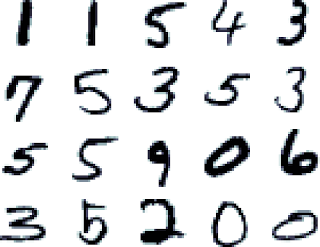
\includegraphics[width=5cm]{figs/mnistexamples}
    \caption{A random sampling of some of the digits in the MNIST handwritten
    digit database}%
    \label{fig:mnistexamples}%
\end{figure}

This problem was chosen because it has significantly many more dimensions than
the 20-dimensional problem from the original OEELM paper
\cite{auerbach2014online} ($28\times28=784$ to be exact), and because the
geometry of the problem is important, a property which HyperNEAT has been shown
to be most suited for \cite{clune2009sensitivity}. 

\section{Multi-output OEELMs}
Since the handwritten digit problem is most efficiently stated as a multi-class
classification problem, modifications had to be made to the original OEELM
method, since it is designed for a single output. 

\subsection{Fitness function}
The original fitness function (Eq.~\ref{eq:oeelmfitness}) relies on there only
being one output neuron, i.e.\ only one connection from a given feature to the
output. To be able to support multi-class classification, the fitness function
for feature $f$ is extended to
\begin{equation}
    fitness(f) = \max \,[\,w_{f \rightarrow o_1},\ldots,w_{f \rightarrow o_n}\,]
    \label{eq:oeelmfitness2}
\end{equation}
where $w_{f \rightarrow o_i}$ is the weight of the connection between the
feature $f$ and output neuron $i$. That is, the fitness of a feature is simply
the weight magnitude of the \emph{largest} connection with the highest such
magnitude. The intuition behind this is that a feature may be very good at
discriminating a single digit, but doesn't contribute towards any of the other
digits (represented by the other neurons). This kind of feature is very
valuable, but if we for example chose to use an average or sum of all the
magnitudes instead, this feature would be scored too low because it does not
contribute much to the rest of the outputs. Using a sum or an average may
incentivize having a similar, high weight to all outputs, which has a low
utility but will score high on fitness.

\subsection{Weight update rule}
Likewise, the weight update rule is modified to support multiple outputs:
\begin{equation}
    \forall f \, \forall i \,(\Delta w_{f \rightarrow o_i} = \eta \times err_i
    \times v_f)
    \label{eq:oeelmdeltaw2}
\end{equation}
where $err_i$ is the difference between the network's output on neuron $i$ and
the correct value for neuron $i$.

\section{Results}
To test the hypothesis that using a NEAT-OEELM could outperform a regular OEELM
on a high dimensional problem domain, a series of experiments were conducted.
The algorithms tested are all online, supervised algorithms. Since they are all
really regression algorithms, the output neuron with the highest value was
chosen as the ``winner''. That is, if for example the third output neuron had
the highest value, this is interpreted as the algorithm classifying that
example as a 2, etcetera (the first output neuron codes for the digit 0).

\subsection{Experimental setup}
%Only the testing set of the MNIST database is used
For each algorithm and parameter set tested, the following steps were performed:
\begin{enumerate}
    \item A randomly chosen example from the testing set of the MNIST database
        is chosen, and presented to the algorithm.
    \item The algorithm makes a prediction, which is recorded.
    \item The algorithm is fed the correct label of the example, and updates its
        weights accordingly.
\end{enumerate}

This process is repeated for as many iterations as was deemed necessary. While
experiments were run with up to 1000000 iterations, as was done in the original
OEELM paper \cite{auerbach2014online}, most graphs in this section is capped at
% TODO revise this number as needed
150000 iterations. This is done because the NEAT-OEELMs use significantly more
time than the original OEELMs due to the added computational complexity, so more
repeated trials was preferred to increased number of iterations. This should not
impact the results, as no algorithms in any experiments showed any improvement
after this number of iterations. All the graphs show the sliding window average
of the error over the last 1000 iterations.

\subsection{Multiple output OEELMs}
First, the original OEELM algorithm, modified to allow for multiple outputs, was
tested.

% TODO INSERT GRAPH SHOWING OELM vs Selection vs OEELM
% TODO Discuss these results.
% TODO Show features

\subsection{NEAT-OEELM compared to OEELM}

% TODO INSERT GRAPH SHOWING OEELM vs NEAT-OEELM (w/o precomplex)
% TODO Discuss these results.
% TODO Show features
% TODO Introduce precomplexification step.
% TODO Show features
% TODO Show results, discuss.

\section{Conclusion}
TODO
\subsection{Further work}
TODO
\section{Source code}
TODO 

\clearpage % To avoid figures inside bibliography
\bibliographystyle{acm}
\bibliography{bibliography}
\end{document}
